\documentclass{article}

% Language setting
% Replace `english' with e.g. `spanish' to change the document language
\usepackage[english]{babel}

% Set page size and margins
% Replace `letterpaper' with `a4paper' for UK/EU standard size
\usepackage[letterpaper,top=2cm,bottom=2cm,left=3cm,right=3cm,marginparwidth=1.75cm]{geometry}

% Useful packages
\usepackage{amsmath}
\usepackage{amssymb}
\usepackage{graphicx}
\usepackage{float}
\usepackage[colorlinks=true, allcolors=blue]{hyperref}
\usepackage{pdfpages}


\title{CSE 102 Notes, Handouts, and Homeworks}
\author{Gary Mejia}
\date{}

\begin{document}
\maketitle

\begin{abstract}
    This is a collection of notes, exercises, and resources for CSE 102, Introduction to Analysis of Algorithms, at UCSC. All this knowledge stems from Patrick Tantalo's Fall 2022 version of CSE 102 but should be applicable to other professor's and other university's version of CSE 102. Everything from handouts to lecture notes to homeworks are here. The document is ordered as follows: notes from each lecture with exercises from discussed handouts, followed by the handouts in alphabetical order, followed by homeworks, ending in homework solutions. Exams are not accessible and thus not here. Linked at the end of this abstract are \href{https://classes.soe.ucsc.edu/cse102/Fall22/}{the CSE 102 website hosted by Patrick Tantalo where lecture recordings can be found}, \href{https://drive.google.com/file/d/1iq3etgnxh6Rh9yO163z4owxypczFhVRB/view?usp=sharing}{the textbook recommended for the course} and \href{https://sites.math.rutgers.edu/~ajl213/CLRS/CLRS.html}{solutions to problems of the textbook}.
\end{abstract}

\section{Lecture 1}

Notes for Lecture 1

\subsection{What functions mean in this class}

Functions such as $g(n)$ and $f(n)$ represent the amount of instructions or operations to complete a task or computation. The names g or f stand for algorithms to complete a task and n is the number of inputs. For example the function f can represent merge sort and g be bubble sort where the input is an array of n elements.

\subsection{Big O Notation}

The statement $f(n) = O(g(n)) $ means the following:

Let g(n) be a function. The set is defined as:
$$ O(g(n)) = \{ f(n) | \exists c > 0 , \exists n_0 > 0, \forall n \geq n_0 : 0 \leq f(n) \leq c \cdot g(n) \}$$ 

In English this means: let $f(n)$ be an element of the set $O(g(n))$ if and only if there exists at least one constant \textbf{c} greater than 0 and there exists at least one constant \textbf{$n_0$} greater than 0, and for all \textbf{n} greater than or equal to \textbf{$n_0$} that makes the inequality true: $0 \leq f(n) \leq c \cdot g(n)$. This is equivalent of saying $f(n)$ grows slower than or the same as $g(n)$. We also say $g(n)$ is the upper asymptotic bound for $f(n)$.

Note: The $\exists$ symbol means only one element needs to exist but does not limit the existence to one element. There can be an infinite amount of elements which means one exists.

\subsubsection{Asymptotic Growth Handout Example 1}

$$10n + 100 = O(n^2 - 40n + 500)$$

We can see for all n greater than or equal to 40 and for a c = 1 the inequality of $10n + 100 \leq n^2 - 40n + 500$ is true. Below is a graphical representation of this example.

\begin{figure}[H]
    \centering
    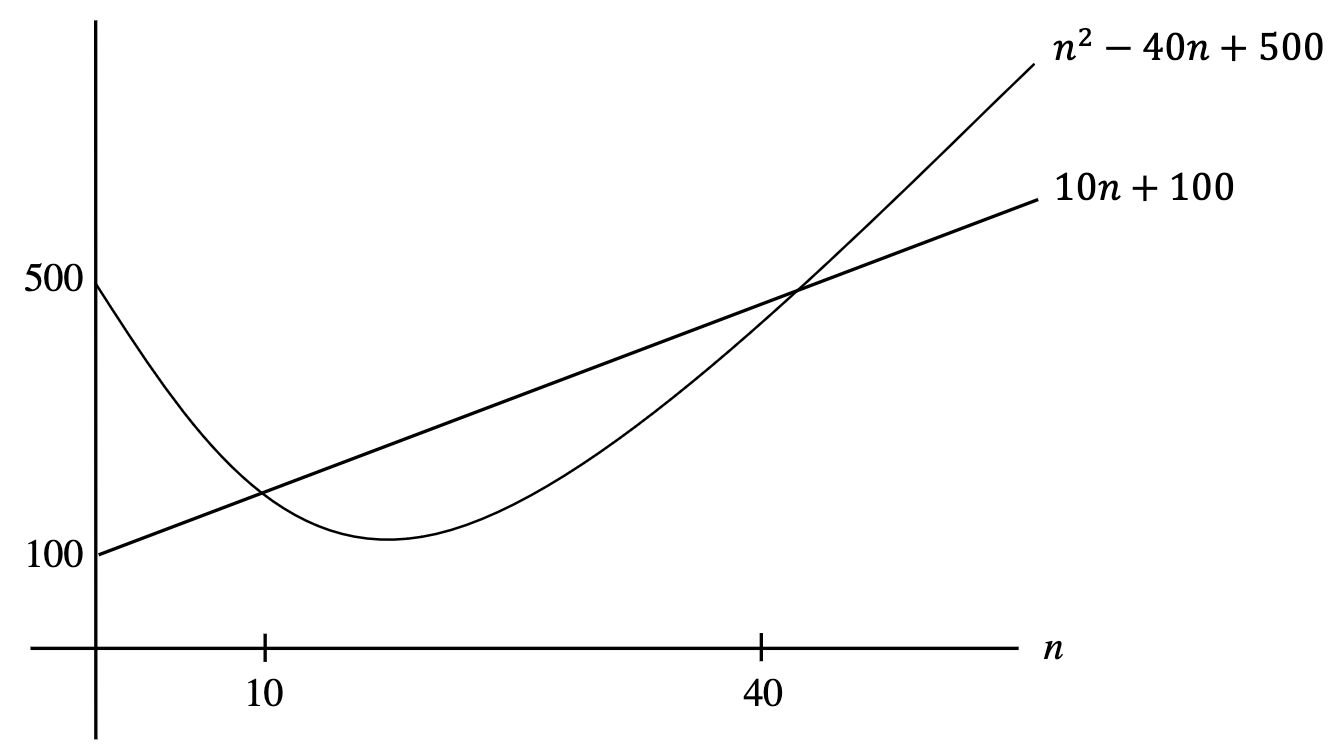
\includegraphics[scale=.4]{Figures/cse102lecture1example1.png}
    \caption{Graphical Representation of Example 1, $n_0 = 40$ and $c = 1$. For all $n \geq n_0$ we see that $n^2 - 40n + 500$ grows faster than $10n + 100$}
    \label{lecture1example1}
\end{figure}

\subsubsection{Generalizations about Big O}
There are two main generalizations we can make of Big O as of now:

\begin{itemize}
    \item 1: \\ an + b = $O(cn^2 +dn + e)$ for constants a,b,c,d,e where a > 0 and c > 0.

    \item 2: \\ If $p(n)$ and $q(b)$ are polynomials with deg(p) $\leq$ deg(q) then $p(n) = O(q(n))$
    
\end{itemize}

\subsection{Big Omega Notation}

The statement $f(n) = \Omega(g(n))$ means the following:

Let g(n) be a function. The set is defined as:
$$ \Omega(g(n)) = \{ f(n) | \exists c > 0 , \exists n_0 > 0, \forall n \geq n_0 : 0 \leq c \cdot g(n) \leq f(n) \}$$ 

In English this means: let $f(n)$ be an element of the set $\Omega(g(n))$ if and only if there exists at least one constant \textbf{c} greater than 0 and there exists at least one constant \textbf{$n_0$} greater than 0, and for all \textbf{n} greater than or equal to \textbf{$n_0$} that makes the inequality true: $0 \leq c \cdot g(n) \leq f(n)$. This is equivalent of saying $f(n)$ grows faster than or the same as $g(n)$. We also say $g(n)$ is the lower asymptotic bound for $f(n)$. Essentially this is the inverse of Big O notation. Below is a graphical representation of Big Omega notation:

\begin{figure}[H]
    \centering
    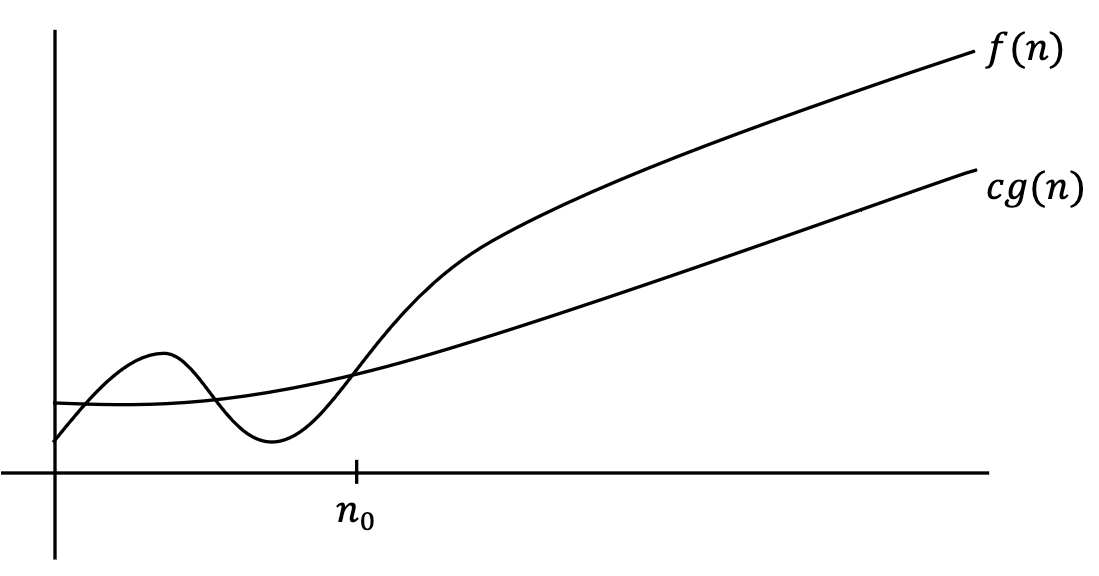
\includegraphics[scale=.4]{Figures/cse102lecture1example2.png}
    \caption{Graphical Representation of Big Omega Notation}
    \label{lecture1example2}
\end{figure}

\subsubsection{Asymptotic Growth Handout Theorem 1 and Proof}

With Big O and Big Omega notation we have the following theorem: 

$$f(n) = O(g(n)) \text{ if and only if } g(n) = \Omega(f(n))$$

The following is its proof:

If $f(n) = O(g(n))$ then there exist at least one positive constant $c_1$ and there exists at least one positive constant $n_1$ such that the inequality $0 \leq f(n) \leq c_1 \cdot g(n)$ is true for all n $\geq n_1$. Let $c_2 = \frac{1}{c_1}$ and $n_2 = n_1$. Multiplying the all sides of the inequality $0 \leq f(n) \leq c_1 \cdot g(n)$ by $c_2$ leads to the inequality $0 \leq c_2 \cdot f(n) \leq g(n)$ which is of the form $g(n) = \Omega(f(n))$. 
Q.E.D 

\subsubsection{Proof of the converse of Theorem 1}

The converse of Theorem 1 is the following:

$$g(n) = \Omega(f(n)) \text{ if and only if } f(n) = O(g(n))$$

The following is its proof:

If $g(n) = \Omega(f(n))$ then there exist at least one positive constant $c_1$ and there exists at least one positive constant $n_1$ such that the inequality $0 \leq c_1 \cdot f(n) \leq g(n)$ is true for all n $\geq n_1$. Let $c_2 = \frac{1}{c_1}$ and $n_2 = n_1$. Multiplying the all sides of the inequality $0 \leq c_1 \cdot f(n) \leq g(n)$ by $c_2$ leads to the inequality $0 \leq f(n) \leq c_2 \cdot g(n)$ which is of the form $f(n) = O(g(n))$. 
Q.E.D 

\subsection{Asymptotically Non-Negative vs Asymptotically Positive}

We say $f(n)$ is asymptotically non-negative if and only if there exists $n_0 > 0$ such that $\forall n \ge n_0$: $f(n) \ge 0$.

We say $f(n)$ is asymptotically positive if and only if there exists $n_0 > 0$ such that $\forall n \ge n_0$: $f(n) > 0$.

\section{Lecture 2}

Notes for Lecture 2

\subsection{Big Theta Notation}

The statement $f(n) = \Theta(g(n))$ means the following:

Let g(n) be a function. The set is defined as:
$$ \Theta(g(n)) = \{ f(n) | \exists c_1 > 0 , \exists c_2 > 0 , \exists n_0 > 0, \forall n \geq n_0 : 0 \leq c_1 \cdot g(n) \leq f(n) \leq c_2 \cdot g(n) \} = O(g(n)) \cap \Omega(g(n))$$ 

In English this means: let $f(n)$ be an element of the set $\Theta(g(n))$ if and only if there exists at least one constant $c_1$ greater than 0 and there exists at least one constant $c_2$ and there exists at least one constant \textbf{$n_0$} greater than 0, and for all \textbf{n} greater than or equal to \textbf{$n_0$} that makes the inequality true: $0 \leq c_1 \cdot g(n) \leq c \cdot f(n) \leq c_2 \cdot g(n)$. We also say $g(n)$ is a tight asymptotic bound for $f(n)$. If we take the ratio of $f(n)$ to $g(n)$ we get the following inequality: $0 \leq c_1 \leq \frac{f(n)}{g(n)} \leq c_2 $.Below is a graphical representation of Big Theta notation:

\begin{figure}[H]
    \centering
    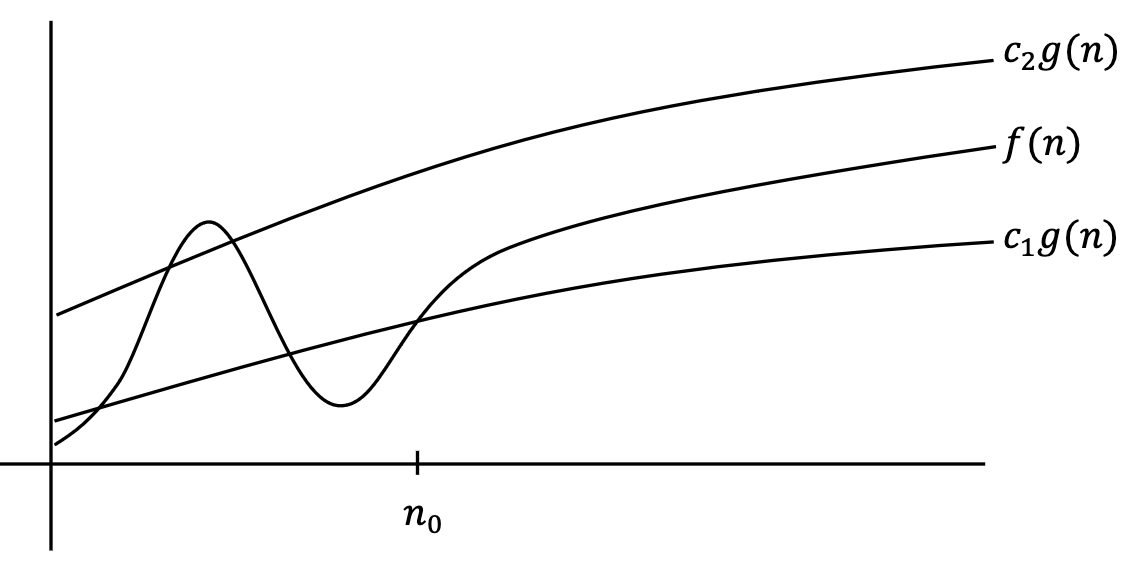
\includegraphics[scale=.4]{Figures/cse102lecture2example1.png}
    \caption{Graphical Notation of Big Theta notation}
    \label{lecture2example1}
\end{figure}

\subsubsection{Asymptotic Growth Handout Exercise 1}

Prove that $f(n) = \Theta(g(n))$ if and only if $g(n) = \Theta(f(n))$

Proof 1:

If $f(n) = \Theta(g(n))$ then $f(n) = O(g(n)) \cap \Omega(g(n))$ we then need to prove that both $g(n) = O(f(n))$ and $g(n) = \Omega(f(n))$ are true. 

If $f(n) = O(g(n))$ then there exists one positive constant $c_0$ and $n_1$ such that the inequality $0 \leq f(n) \leq c_0 \cdot g(n)$ for all n $\geq n_1$. Let positive constant $c_2 = \frac{1}{c_0}$ and $n_2 = n_1$. Multiplying all sides of the previous inequality gets the inequality $0 \leq c_2 \cdot f(n) \leq g(n)$ which is $g(n) = \Omega(f(n))$.

If $f(n) = \Omega(g(n))$ then there exists one positive constant $c_0$ and $n_1$ such that the inequality $0 \leq c_0 \cdot g(n) \leq f(n)$ for all n $\geq n_1$. Let positive constant $c_1 = \frac{1}{c_0}$ and $n_2 = n_1$. Multiplying all sides of the previous inequality gets the inequality $0 \leq g(n) \leq c_1 \cdot f(n)$ which is $g(n) = O(f(n))$.

Since both $g(n) = O(f(n))$ and $g(n) = \Omega(f(n))$ then it is proven that $g(n) = \Theta(f(n))$. Q.E.D

\subsubsection{Asymptotic Growth Handout Exercise 2}

Let $g(n)$ be any function, and c > 0. Prove the following: (a) $c \cdot g(n) = O(g(n))$, (b) $c \cdot g(n) = \Omega(g(n))$,(c) $c \cdot g(n) = \Theta(g(n))$. 

Part A:

If $c \cdot g(n) = O(g(n))$ then there exists at least one positive constant $c_n$ and one positive constant $n_0$ such that, for all n $\geq n_0$ make the following inequality true: $0 \leq c \cdot g(n) \leq c_n \cdot g(n)$. If $g(n)$ is asymptotic positive, we can divide the inequality by $g(n)$ to get the following inequality: $0 \leq c \leq c_n$. Thus for any $c_n \geq c$ we see that $c \cdot g(n) = O(g(n))$. Q.E.D

Part B:

If $c \cdot g(n) = \Omega(g(n))$ then there exists at least one positive constant $c_n$ and one positive constant $n_0$ such that, for all n $\geq n_0$ make the following inequality true: $0 \leq c_n \cdot g(n) \leq c \cdot g(n)$. If $g(n)$ is asymptotic positive, we can divide the inequality by $g(n)$ to get the following inequality: $0 \leq c_n \leq c$. Thus for any $c_n \leq c$ we see that $c \cdot g(n) = \Omega(g(n))$. Q.E.D

Part C:

If $c \cdot g(n) = \Theta(g(n))$ then there exists at least one positive constant $c_n$, $c_m$, and one positive constant $n_0$ such that, for all n $\geq n_0$ make the following inequality true: $0 \leq c_m \cdot g(n) \leq c \cdot g(n) \leq c_n \cdot g(n)$. If $g(n)$ is asymptotic positive, we can divide the inequality by $g(n)$ to get the following inequality: $0 \leq c_m \leq c \leq c_n$. Thus for any $c_n \geq c$ and any $c_m \leq c$ we see that $c \cdot g(n) = \Theta(g(n))$. Q.E.D

\subsubsection{Asymptotic Growth Handout Example 2}

Prove that $\sqrt{n + 10} = \Theta(\sqrt{n})$

We must find at least one set of positive constants $c_1$,$c_2$,$n_0$ such that the following inequality holds true: $0 \leq c_1 \cdot \sqrt{n} \leq \sqrt{n + 10}\leq c_2 \cdot \sqrt{n}$ for all n $\geq n_0$. Let $c_1 = 1$, $c_2 = \sqrt{2}$, and $n_0 = 10$. Then if $n \geq n_0$, the following statements are true: $-10 \leq 0$ and $10 \leq n$. Therefore we have the following true statements: $-10 \leq (1-1)n$ and $10 \leq (2-1)n$ Replacing 1 for $c_1^2$ and 2 for $c_2^2$ we get the following statements: $-10 \leq (1-c_1^2)n$ and $10 \leq (c_2^2 -1)n$. Doing some algebra on both statements we get the following: $c_1^2 \cdot n\leq n + 10$ and $n +10 \leq c_2^2 \cdot n$. Combining both statements into one inequality gets the following inequality: $c_1^2 \cdot n \leq n + 10 \leq c_2^2 \cdot n$. Since both $c_1$ and $c_2$ are positive numbers we get the following inequality: $0 \leq c_1^2 \cdot n \leq n + 10 \leq c_2^2 \cdot n$. Finally we root the entire inequality to get $0 \leq c_1 \cdot \sqrt{n} \leq \sqrt{n + 10} \leq c_2 \cdot \sqrt{n}$ which is the form $\sqrt{n + 10} = \Theta(\sqrt{n})$. Q.E.D

Note: For this proof and others like it, working backwards is a good way to find the values needed for the proof.

\subsubsection{Asymptotic Growth Handout Exercise 3}

Let a,b be real numbers with $b > 0$. Prove directly from the definition that $(n + a)^b = \Omega(g(n^b))$.

$$0 \leq c_1 \cdot n^b \leq (n + a)^b \leq c_2 \cdot n^b$$
$$\text{Since } n > |a| \text{ we can state the following:}$$
$$n + a \leq n + |a| \leq 2n$$
$$\text{If we bound a such that } |a| \leq \frac{1}{3}n \text{ we can state the following:}$$
$$\frac{1}{3}n \leq n - |a| \leq n + a$$
$$\text{Thus when } n \geq 3|a| \text{ then:}$$
$$\frac{1}{3}n \leq n + a \leq 2n$$
$$\text{Raising the inequality by b gets the following:}$$
$$(\frac{1}{3}n)^b \leq (n + a) \leq 2^b n^b$$
$$\text{Thus } n_0 = 3|a|, c_1 = (\frac{1}{3})^b ,c_2 = 2^b$$
\href{http://hscc.cs.nthu.edu.tw/~sheujp/lecture_note/14algorithm/Chap\%203_HW.pdf}{Q.E.D}

\subsubsection{Asymptotic Growth Handout Theorem 2 and Proof}

If $h(n)$ = $O(g(n))$ and if $ f(n) \leq h(n) $ for all sufficiently large n, then $f(n) = O(g(n))$.

Proof:
If $h(n) = O(g(n))$ then there exists at least one positive constant c and $n_0$ such that the following inequality holds true for all $n \geq n_0$: $0 \leq h(n) \leq c \cdot g(n)$. Since $f(n) \leq h(n)$ for all $n \geq n_2$, then $n \geq max(n_1 , n_2)$ holds and the following inequality is true: $0 \leq f(n) \leq h(n) \leq c \cdot g(n)$. Therefore $f(n) = O(g(n))$. Q.E.D

\subsubsection{In Class Theorem and Proof}

If $h(n)$ = $\Omega(g(n))$ and if $ f(n) \geq h(n) $ for all sufficiently large n, then $f(n) = \Omega(g(n))$.

If $h(n) = \Omega(g(n))$ then there exists at least one positive constant c and $n_0$ such that the following inequality holds true for all $n \geq n_0$: $0 \leq c \cdot g(n) \leq h(n)$. Since $f(n) \geq h(n)$ for all $n \geq n_2$, then $n \geq max(n_1 , n_2)$ holds and the following inequality is true: $0 \leq c \cdot g(n) \leq h(n) \leq f(n) $. Therefore $f(n) = \Omega(g(n))$. Q.E.D

\subsubsection{Asymptotic Growth Handout Exercise 4}

Prove that if $h_1(n) \leq f(n) \leq h_2(n)$ for all sufficiently large n, where $h_1 = \Omega(g(n))$ and $h_2(n) = O(g(n))$, then $f(n) = \Theta(g(n))$.

Proof:
$$\text{We note that the following two statements are true:}$$
$$h_1(n) \leq f(n) \text{ and } f(n) \leq h_2(n)$$
$$\text{Since } h_1(n) \leq f(n) \text{ and } h_1(n) = \Omega(g(n)) \text{ we can prove that } f(n) = \Omega(g(n)) \text{:}$$
If $h(n) = \Omega(g(n))$ then there exists at least one positive constant c and $n_0$ such that the following inequality holds true for all $n \geq n_0$: $0 \leq c \cdot g(n) \leq h(n)$. Since $f(n) \geq h(n)$ for all $n \geq n_2$, then $n \geq max(n_1 , n_2)$ holds and the following inequality is true: $0 \leq c \cdot g(n) \leq h(n) \leq f(n) $. Therefore $f(n) = \Omega(g(n))$. 
$$\text{Furthermore we can prove that since } f(n) \leq h_2(n) \text{ and } h_2(n) = O(g(n)) \text{: } f(n) = O(g(n)).$$
If $h(n) = O(g(n))$ then there exists at least one positive constant c and $n_0$ such that the following inequality holds true for all $n \geq n_0$: $0 \leq h(n) \leq c \cdot g(n)$. Since $f(n) \leq h(n)$ for all $n \geq n_2$, then $n \geq max(n_1 , n_2)$ holds and the following inequality is true: $0 \leq f(n) \leq h(n) \leq c \cdot g(n)$. Therefore $f(n) = O(g(n))$. 
$$\text{Since we have proven that both } f(n) = \Omega(g(n)) \text{ and } f(n) = O(g(n)) \text{ then } f(n) = \Theta(g(n)).$$
Q.E.D

\subsubsection{Asymptotic Growth Handout Example 3}

Let $k \geq 1$ be a fixed integer. Proof that $\Sigma_{i=1}^{n} (i^k) = \Theta(n^{k+1})$.
Proof:
Observe by Asymptotic Growth Handout Theorem 2, $\Sigma_{i=1}^{n} (i^k) \leq \Sigma_{i=1}^{n} (n^k) = n \cdot n^k = n^{k+1} = O(n^{k+1}).$ To get the lower bound of $\Theta(n^{k+1})$, we do the following:

$$\Sigma_{i=1}^{n} (i^k) \geq \Sigma_{i=ceil(\frac{n}{2})}^{n} (i^k)$$
$$\geq \Sigma_{i=ceil(\frac{n}{2})}^{n} ((ceil(\frac{n}{2})^k)$$
$$= (n - ceil(\frac{n}{2}) + 1) \cdot ((ceil(\frac{n}{2})^k)$$
$$= (floor(\frac{n}{2}) + 1) \cdot ((ceil(\frac{n}{2})^k))$$
$$> (\frac{n}{2} -1 + 1) \cdot (\frac{n}{2})^k$$
$$> (\frac{n}{2} -1 + 1) \cdot (\frac{n}{2})^k$$
$$= (\frac{n}{2}) \cdot (\frac{n}{2})^k$$
$$= (\frac{1}{2})^{k+1} \cdot n^{k+1}$$
$$ = \Omega(n^{k+1})$$
Q.E.D

This proof is consistent with the summation $\Sigma_{i=1}^{n} i = \frac{n(n+1)}{2} = \Omega(n^2)$.

\subsubsection{Asymptotic Growth Handout Exercise 5}

Prove that $\Sigma_{i=1}^{n} \Theta(i) = \Theta(n^2)$. 

$$\text{Let us define the following functions } h_1(n) \text{ and } h_2(n) \text{ such that } h_1(n) = \Omega(n^2) \text{ and } h_2(n) = O(n^2).$$
$$\text{Also let the following inequality be true: } h_1(n) \leq f(n) \leq h_2(n) \text{ where } c_1 > 0, c_2 > 0\text{ thus we can say:}$$
$$c_1 \cdot \Sigma_{i=1}^{n} h_1(i) \leq \Sigma_{i=1}^{n} f(i) \leq c_2 \cdot \Sigma_{i=1}^{n} h_2(i) $$
$$\text{By the definition of a linear summation:}$$
$$c_1 \cdot \frac{n(n+1)}{2} \leq \Sigma_{i=1}^{n} f(i) \leq c_2 \cdot \frac{n(n+1)}{2} $$
$$\text{Thus we can say } \Sigma_{i=1}^{n} f(i) = \Theta(n^2).$$
Q.E.D

\subsection{Little o Notation}

The statement $f(n) = o(g(n)) $ means the following:

Let g(n) be a function. The set is defined as:
$$ o(g(n)) = \{ f(n) | \forall c > 0 , \exists n_0 > 0, \forall n \geq n_0 : 0 \leq f(n) < c \cdot g(n) \}$$ 

Remember that $f(n) = o(g(n)) = \{ f(n) | \exists c > 0 , \exists n_0 > 0, \forall n \geq n_0 : 0 \leq f(n) \leq c \cdot g(n) \}$

In English this means: let $f(n)$ be an element of the set $o(g(n))$ if there exists at least one constant \textbf{$n_0$} greater than 0, and for all \textbf{n} greater than or equal to \textbf{$n_0$} and for all c greater than 0 that makes the inequality true: $0 \leq f(n) \leq c \cdot g(n)$. This is equivalent of saying $f(n)$ strictly grows slower than $g(n)$. We also say $g(n)$ is the STRICT upper asymptotic bound for $f(n)$. We see that $o(g(n))$ is a subset of $O(g(n))$.

\subsubsection{Asymptotic Growth Handout Lemma 1 and Proof}

$f(n) = o(g(n))$ if and only if $\lim_{n \rightarrow \infty} \frac{f(n)}{g(n)} = 0 $.

Proof:
See that $f(n) = o(g(n))$ if for all c greater than c, there exists at least one $n_0$, for all $n \geq n_0$ such that the inequality $0 \leq \frac{f(n)}{g(n)} < c$ holds true. That inequality is the limit definition of $f(n) = o(g(n))$.

\section{Lecture 3}

Notes for Lecture 3

\subsection{Little o Notation Cont.}

\subsubsection{Asymptotic Growth Handout Example 4}
Prove $\ln{n} = o(n)$.
Proof:
$$\lim_{n \rightarrow \infty} \frac{\ln{(n)}}{n}$$
$$\text{By L'Hopital's Rule}$$
$$\lim_{n \rightarrow \infty} \frac{1}{n} = 0$$
Q.E.D

\subsubsection{Lecture 3 In Class Exercise 1}
Prove $\ln{(n)} = o(n^k)$ for all $k > 0$.
Proof:
$$\lim_{n \rightarrow \infty} \frac{\ln{(n)}}{n^k}$$
$$\text{By L'Hopital's Rule}$$
$$=\lim_{n \rightarrow \infty} \frac{1}{kn^{k-1}} = 0$$
Q.E.D

\subsubsection{Lecture 3 In Class Exercise 2}
Prove ($\ln{(n)})^m = o(n^k)$ for all $k > 0$ and for all $m \geq 0$.
$$\lim_{n \rightarrow \infty} \frac{(\ln{(n)})^m}{n^k}$$
$$\text{Let } n^k = e^{k \cdot \ln{(n)}}$$
$$=\lim_{n \rightarrow \infty} \frac{(\ln{(n)})^m}{e^{k \cdot \ln{(n)}}}$$
$$\text{By L'Hopital's Rule}$$
$$=\lim_{n \rightarrow \infty} \frac{ \frac{m}{n} \cdot (\ln{(n)})^{m-1}}  { \frac{k}{n} \cdot e^{k \cdot \ln{(n)}}} = 0$$
$$\text{By L'Hopital's Rule Again an m amount of times}$$
$$=\lim_{n \rightarrow \infty} \frac{ m! }  { k^m \cdot e^{k \cdot \ln{(n)}}} = 0$$
Q.E.D

\subsubsection{Lecture 3 In Class Exercise 3}
Prove $(\log_{b}{(n)})^m = o(n^k)$ for all $k > 0$ and for all $m \geq 0$ and for all $b \geq 1$.
$$\lim_{n \rightarrow \infty} \frac{(\log_{b}{(n)})^m}{n^k}$$
$$\text{Let } n^k = b^{k \cdot \log_{b}{(n)}}$$
$$=\lim_{n \rightarrow \infty} \frac{(\log_{b}{(n)})^m}{b^{k \cdot \log_{b}{(n)}}}$$
$$\text{By L'Hopital's Rule}$$
$$= \lim_{n \rightarrow \infty} \frac{ \frac{m}{n\ln{(b)}} \cdot (\log_{b}{(n)})^{m-1}}{ \frac{k \cdot \ln{(b)}}{n\ln{(b)}} \cdot b^{k \cdot \log_{b}{(n)}}}$$
$$= \frac{mk}{\ln{(b)}} \cdot \lim_{n \rightarrow \infty} \frac{(\log_{b}{(n)})^{m-1}}{ b^{k \cdot\log_{b}{(n)}}}$$
$$\text{By L'Hopital's Rule Again an m amount of times}$$
$$= \frac{m!k^m}{\ln{(b)}^m} \cdot \lim_{n \rightarrow \infty} \frac{1}{ b^{k \cdot\log_{b}{(n)}}} = 0 $$
Q.E.D

\subsubsection{Asymptotic Growth Handout Example 5}
Prove $n^k = o(e^n)$ for all k in the real numbers and all $ b > 1$.
$$\lim_{n \rightarrow \infty} \frac{n^k}{e^n}$$
$$\text{Apply L'Hopital's Rule n times to get:}$$
$$=\lim_{n \rightarrow \infty} \frac{k!}{e^n}=0$$
Q.E.D

\subsubsection{Lecture 3 In Class Exercise 4}
Prove $n^k = o(b^n)$ for all k in the real numbers.
$$\lim_{n \rightarrow \infty} \frac{n^k}{b^n}$$
$$\text{Apply L'Hopital's Rule n times to get:}$$
$$=\lim_{n \rightarrow \infty} \frac{k!\ln{(b)}^k}{b^n}=0$$
Q.E.D

\subsubsection{Asymptotic Growth Handout Exercise 6}
Prove that $o(g(n)) \cap \Omega(g(n)) = \emptyset$
$$f(n) = o(g(n)) \cap \Omega(g(n)) \text{ if for all } c > 0, \exists n_0 > 0, n \geq n_0 \text{ the inequality below is true }$$
$$0 \leq c \cdot g(n) \leq f(n) < c \cdot g(n)$$
$$\text{However if } c = 1 \text{ the inequality becomes the following:}$$
$$0 \leq g(n) \leq f(n)  < g(n)$$
$$\text{The inequality above can never be satisfied thus } o(g(n)) \cap \Omega(g(n)) = \emptyset$$
Q.E.D

\subsection{Little Omega Notation}

The statement $f(n) = \Omega(g(n))$ means the following:

Let g(n) be a function. The set is defined as:
$$ \omega(g(n)) = \{ f(n) | \forall c > 0 , \exists n_0 > 0, \forall n \geq n_0 : 0 \leq c \cdot g(n) < f(n) \}$$ 

In English this means: let $f(n)$ be an element of the set $\Omega(g(n))$ if and for all constants \textbf{c} greater than 0 and there exists at least one constant \textbf{$n_0$} greater than 0, and for all \textbf{n} greater than or equal to \textbf{$n_0$} that makes the inequality true: $0 \leq c \cdot g(n) < f(n)$. This is equivalent of saying $f(n)$ strictly grows faster than $g(n)$. We also say $g(n)$ is the STRICT lower asymptotic bound for $f(n)$. We see that $\omega(g(n))$ is a subset of $\Omega(g(n))$.

\subsubsection{Asymptotic Growth Handout Exercise 7}
Prove $f(n) = \omega(g(n))$ if and only if $\lim_{n \rightarrow \infty} \frac{f(n)}{g(n)} = \infty $. Also prove $\omega(g(n)) \cap O(g(n)) = \emptyset$.

See that $f(n) = \omega(g(n))$ if for all c greater than c, there exists at least one $n_0$, for all $n \geq n_0$ such that the inequality $0 < \frac{f(n)}{g(n)} \leq \infty $ holds true. That inequality is the limit definition of $f(n) = \omega(g(n))$.

$$f(n) = \omega(g(n)) \cap O(g(n)) \text{ if for all } c > 0, \exists n_0 > 0, n \geq n_0 \text{ the inequality below is true }$$
$$0 \leq c \cdot g(n) < f(n) \leq c \cdot g(n)$$
$$\text{However if } c = 1 \text{ the inequality becomes the following:}$$
$$0 \leq g(n) < f(n)  \leq g(n)$$
$$\text{The inequality above can never be satisfied thus } \omega(g(n)) \cap O(g(n)) = \emptyset$$
Q.E.D

With all the order of functions proven so far we can picture them as the Venn diagram below:

\begin{figure}[H]
    \centering
    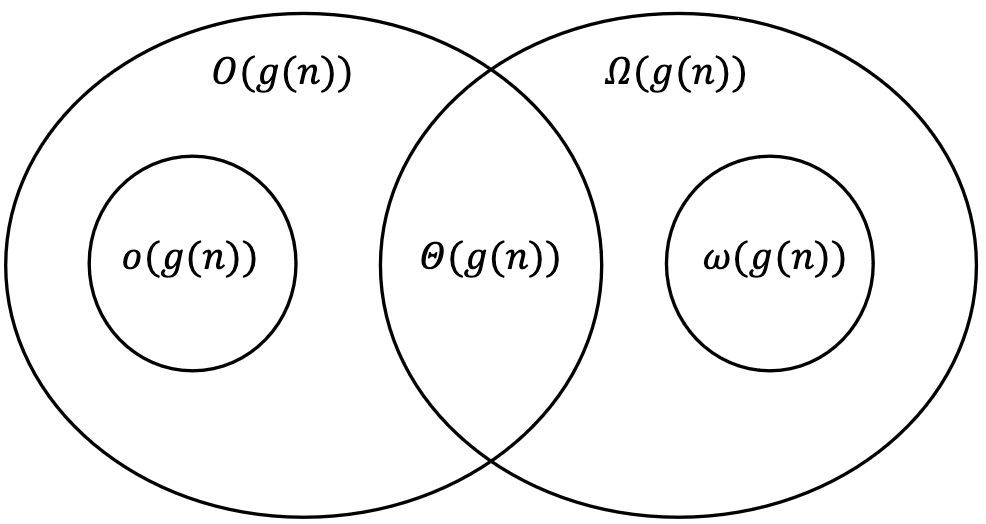
\includegraphics[scale=.4]{Figures/cse102lecture3example1.png}
    \caption{Venn Diagram of all order of functions}
    \label{lecture3example1}
\end{figure}

\subsubsection{Asymptotic Growth Handout Theorem 3 and Proof}
If $\lim_{n \rightarrow \infty} \frac{f(n)}{g(n)} = L$, where $0 \leq L < \infty$, then $f(n) = O(g(n))$. Note: The converse is false.

Proof: 
The limit statement says $\forall \epsilon > 0, \exists n_0 > 0, \forall n \geq n_0 : \big| \frac{f(n)}{g(n)} - L \big| < \epsilon$. ince this holds for all $\epsilon$, we may set $\epsilon$ = 1. Then there exists a positive $n_0$ such that for all $n \geq n_0$:
$$\big| \frac{f(n)}{g(n)} - L \big| < 1$$
$$\therefore  -1 < \frac{f(n)}{g(n)} - L < 1$$
$$\therefore \frac{f(n)}{g(n)}  <L + 1$$
$$\therefore f(n) < (L + 1) \cdot g(n)$$
$$\text{Let } c = (L + 1) \text{ which yields the  definition for } f(n) = O(g(n)).$$
Q.E.D

\subsubsection{Asymptotic Growth Handout Theorem 4 and Proof}
If $\lim_{n \rightarrow \infty} \frac{f(n)}{g(n)} = L$, where $0 < L \leq \infty$, then $f(n) = \Omega(g(n))$. Note: The converse is false.

Proof: 
The limit statement says $\forall \epsilon > 0, \exists n_0 > 0, \forall n \geq n_0 : \big| \frac{g(n)}{f(n)} - L \big| < \epsilon$. ince this holds for all $\epsilon$, we may set $\epsilon$ = 1. Then there exists a positive $n_0$ such that for all $n \geq n_0$:
$$\big| \frac{g(n)}{f(n)} - L \big| < 1$$
$$\therefore  -1 < \frac{g(n)}{f(n)} - L < 1$$
$$\therefore \frac{g(n)}{f(n)}  <L + 1$$
$$\therefore \frac{g(n)}{(L + 1)} < f(n)$$
$$\text{Let } c = \frac{1}{(L + 1)} \text{ which yields the  definition for } f(n) = \Omega(g(n)).$$
Q.E.D

\subsubsection{Asymptotic Growth Handout Theorem 5 and Proof as Exercise 8}

Prove that if $\lim_{n \rightarrow \infty} \frac{f(n)}{g(n)} = L$, where $) < L < \infty$, then $f(n) = \Theta(g(n))$.

The limit statement says $\forall \epsilon > 0, \exists n_0 > 0, \forall n \geq n_0 : \big| \frac{f(n)}{g(n)} - L \big| < \epsilon$. ince this holds for all $\epsilon$, we may set $\epsilon$ = 1. Then there exists a positive $n_0$ such that for all $n \geq n_0$:
$$\big| \frac{f(n)}{g(n)} - L \big| < 1$$
$$\therefore  -1 < \frac{f(n)}{g(n)} - L < 1$$
$$\therefore \frac{f(n)}{g(n)}  <L + 1$$
$$\therefore {f(n)} < (L+1) \cdot g(n)$$
$$\text{Let } c_1 = {(L + 1)} \text{ which yields the  definition for } f(n) = O(g(n)).$$
$$\text{We can use the same limit definition to find a constant} c_2 \text{ using the same } \epsilon = 1$$
$$\big| \frac{g(n)}{f(n)} - L \big| < 1$$
$$\therefore  -1 < \frac{g(n)}{f(n)} - L < 1$$
$$\therefore \frac{g(n)}{f(n)}  <L + 1$$
$$\therefore \frac{g(n)}{(L + 1)} < f(n)$$
$$\text{Let } c_2 = \frac{1}{(L + 1)} \text{ which yields the  definition for } f(n) = \Omega(g(n)).$$
$$\text{Thus with these two constants are in between 0 and infinity, we get the definition for } f(n) = \Theta(g(n)).$$
Q.E.D

\subsubsection{Asymptotic Growth Handout Example A}

Let $g(n) = n$ and $f(n) = (1 + \sin(n)) \cdot n$

\begin{figure}[H]
    \centering
    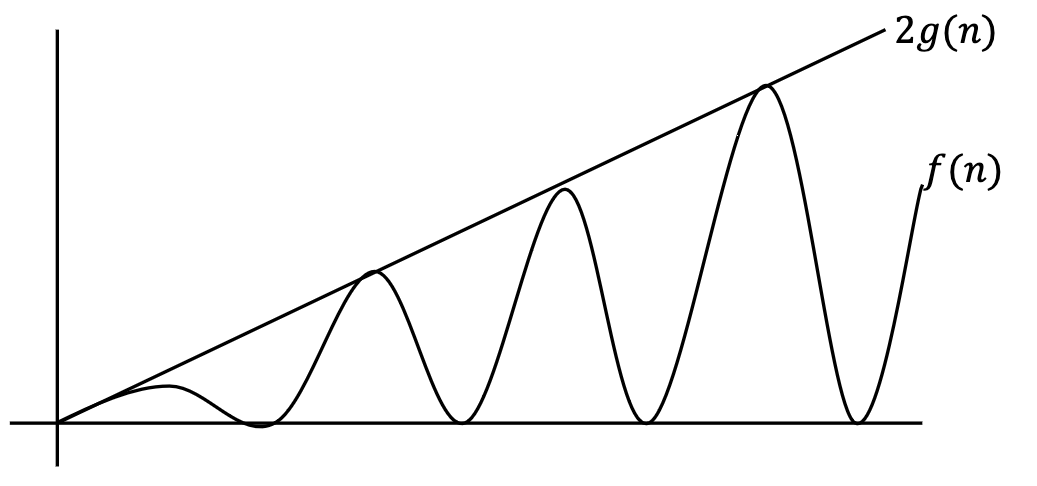
\includegraphics[scale=.4]{Figures/cse102lecture3exampleA.png}
    \caption{Example A}
    \label{lecture3exampleA}
\end{figure}

As shown above, $f(n) = O(g(n))$ and there are no positive non-zero constants $c_1$ and $c_2$ that make the following inequality true: $0 \leq c_1 \cdot g(n) \leq f(n) \leq c_2 \cdot g(n)$ thus $f(n) \notin \Theta(g(n))$. If we take the ratio of $f(n)$ to $g(n)$ we see $\frac{f(n)}{g(n)} = 1 + \sin(n)$ which has no limit. Thus $f(n) \in O(g(n)) - \Theta(g(n)) - o(g(n))$.

\subsection{Limit Rule Exceptions}

\subsubsection{Asymptotic Growth Handout Example A}

Let $g(n) = n$ and $f(n) = (2 + \sin(n)) \cdot n$

\begin{figure}[H]
    \centering
    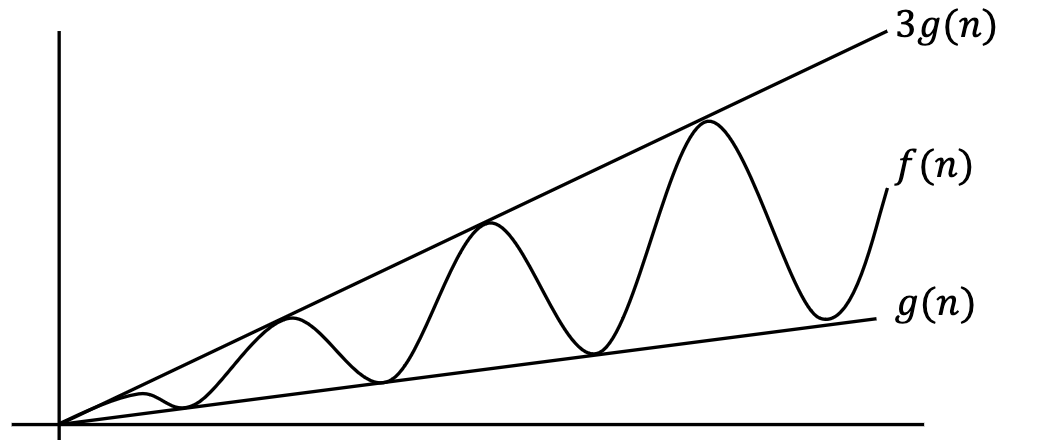
\includegraphics[scale=.4]{Figures/cse102lecture3exampleB.png}
    \caption{Example A}
    \label{lecture3exampleB}
\end{figure}

As shown above, $f(n) = \Theta(g(n))$. If we take the ratio of $f(n)$ to $g(n)$ we see $\frac{f(n)}{g(n)} = 2 + \sin(n)$ which has no limit. Thus $f(n) \in \Theta(g(n)) - \Theta(g(n))$ with no limit.



\subsubsection{Asymptotic Growth Handout Exercise 9 and Example C}

Find functions $f(n)$ and $h(n)$ such that $f(n) \in \Omega(g(n)) - \Theta(g(n))$, but $\lim_{n \rightarrow \infty} \frac{f(n))}{g(n))}$ does not exist, so that $f(n) \neq \omega(g(n))$. 

Let $g(n) = n$ and $f(n) = n^2 \cdot \sin(n)$

If $c = 1$ and $n_0 = 1$ then for all $n \geq n_0$ the inequality: $0 \leq c \cdot g(n) \leq f(n)$ holds, thus $f(n) = \Omega(g(n))$. However there are no positive constants $c_1$ and $c_2$ such that the following inequality: $0 \leq c_1 \cdot g(n) \leq f(n) \leq c_2 \cdot g(n)$ holds, thus $f(n) \neq \Theta(g(n))$. Additionally if we take the ratio of $f(n)$ to $g(n)$ we get $\frac{f(n)}{g(n)} = n \cdot sin(n)$ which has no limit thus $f(n) \in \Omega(g(n)) - \Theta(g(n)) - \omega(g(n))$. 

The examples above show that the full sets of $\omega$, o, and some sets of $\Theta$ are categorized by the limit rules, the full sets of $\Omega$, O and $\Theta$ are not. The following venn diagram appears:

\begin{figure}[H]
    \centering
    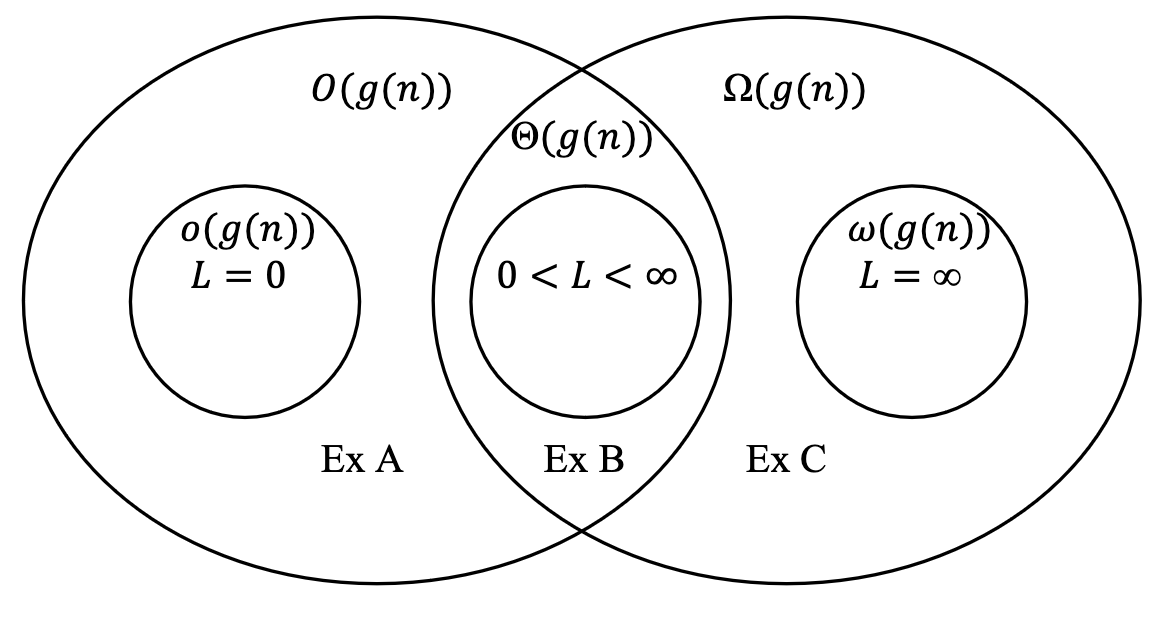
\includegraphics[scale=.4]{Figures/cse102lecture3figure1.png}
    \caption{Venn Diagram of all order of functions with limits}
    \label{lecture3figure1}
\end{figure}

\subsection{Limit Rule Practice}

\subsubsection{Asymptotic Growth Handout Exercise 10}
Use the following limit rules to prove the following:

\subsubsection{Exercise 10A}

Prove $n\cdot ln(n) = o(n^2)$ and $n \cdot \log_b(n) = o(n^2), b > 0$

$$\lim_{n \rightarrow \infty} \frac{n\cdot ln(n)}{n^2} $$
$$\lim_{n \rightarrow \infty} \frac{ln(n)}{n} $$
$$\lim_{n \rightarrow \infty} \frac{1}{n} = 0$$
$$n\cdot ln(n) = o(n^2) \text{ Q.E.D}$$
$$\textbf{AND}$$
$$\lim_{n \rightarrow \infty} \frac{n\cdot \log_b(n)}{n^2} $$
$$\lim_{n \rightarrow \infty} \frac{\log_b(n)}{n} $$
$$\lim_{n \rightarrow \infty} \frac{1}{ln(b)\cdot n} = 0$$
$$n\cdot \log_b(n) = o(n^2) \text{Q.E.D}$$

\subsubsection{Exercise 10B}
Prove $n^5 \cdot 2^n = \omega(n^{10})$

$$\lim_{n \rightarrow \infty} \frac{n^{5} \cdot 2^n}{n^{10}}$$
$$\lim_{n \rightarrow \infty} \frac{2^n}{n^5}$$
$$\lim_{n \rightarrow \infty} \frac{\ln(2) \cdot 2^n}{5n^4} $$
$$\text{Apply L'Hopital Rule 4 more times}$$
$$\lim_{n \rightarrow \infty} \frac{\ln^5(2) \cdot 2^n}{120} = \infty$$
$$n^5 \cdot 2^n = \omega(n^{10}), \text{ Q.E.D}$$

\subsubsection{Exercise 10C}

Prove if $P(n)$ is a polynomial of degree $k \geq 0$, then $P(n) = \Theta(n^k)$.

$$\lim_{n \rightarrow \infty} \frac{P(n)}{n^k}$$
$$\text{Apply L'Hopital Rule k times}$$
$$\lim_{n \rightarrow \infty} \frac{k!}{k!} = 1$$
$$ P(n) = \Theta(n^{k}), \text{ Q.E.D}$$

\subsubsection{Exercise 10D}

For any positive real numbers $\alpha$ and $\beta$: $n^{\alpha} = o(n^{\beta})$ iff $\alpha < \beta$,$n^{\alpha} = \Theta(n^{\beta})$ iff $\alpha = \beta$,$n^{\alpha} = \omega(n^{\beta})$ iff $\alpha > \beta$.

$$\text{If } \alpha < \beta \text{ then let }\alpha = \beta - 1, \text{ then} $$
$$\lim_{n \rightarrow \infty} \frac{n^{\beta - 1}}{n^{\beta}}$$
$$\text{Apply L'Hopital Rule } \beta - 1 \text{ times}$$
$$\lim_{n \rightarrow \infty} \frac{{(\beta - 1)}!}{n} = 0$$
$$n^{\alpha} = o(n^{\beta}) \text{ iff } \alpha < \beta \text{ Q.E.D}$$

$$\text{If } \alpha = \beta \text{ then let }\alpha = \beta, \text{ then} $$
$$\lim_{n \rightarrow \infty} \frac{n^{\beta}}{n^{\beta}}$$
$$\text{Apply L'Hopital Rule } \beta \text{ times}$$
$$\lim_{n \rightarrow \infty} \beta = \beta $$
$$n^{\alpha} = \Theta(n^{\beta}) \text{ iff } \alpha = \beta \text{ Q.E.D}$$

$$\text{If } \alpha > \beta \text{ then let }\alpha = \beta + 1, \text{ then} $$
$$\lim_{n \rightarrow \infty} \frac{n^{\beta + 1}}{n^{\beta}}$$
$$\text{Apply L'Hopital Rule } \beta \text{ times}$$
$$\lim_{n \rightarrow \infty} n = \infty$$
$$n^{\alpha} = \omega(n^{\beta}) \text{ iff } \alpha > \beta \text{ Q.E.D}$$

\subsubsection{Exercise 10E}

For any positive real numbers $\alpha$ and $\beta$: $\alpha^n = o(\beta^n)$ iff $\alpha < \beta$,$\alpha^n = \Theta(\beta^n)$ iff $\alpha = \beta$,$\alpha^n = \omega(\beta^n)$ iff $\alpha > \beta$.

$$\lim_{n \rightarrow \infty} \frac{\alpha^n}{{\beta}^n}$$
$$\lim_{n \rightarrow \infty} (\frac{\alpha}{\beta})^n$$
$$\text{If } \alpha < \beta \text{ then let }\alpha = \beta - 1, \text{ then} $$
$$\lim_{n \rightarrow \infty} (\frac{\beta - 1}{\beta})^n = 0$$
$$\text{Since } 0 < \frac{\alpha}{\beta} < 1 \text{ this is an exponential function with a base between 0 and 1 thus this limit is 0}$$
$$n^{\alpha} = o(n^{\beta}) \text{ iff } \alpha < \beta \text{ Q.E.D}$$

$$\lim_{n \rightarrow \infty} \frac{\alpha^n}{{\beta}^n}$$
$$\lim_{n \rightarrow \infty} (\frac{\alpha}{\beta})^n$$
$$\text{If } \alpha < \beta \text{ then let }\alpha = \beta, \text{ then} $$
$$\lim_{n \rightarrow \infty} (\frac{\beta}{\beta})^n = 1$$
$$n^{\alpha} = \Theta(n^{\beta}) \text{ iff } \alpha < \beta \text{ Q.E.D}$$

$$\lim_{n \rightarrow \infty} \frac{\alpha^n}{{\beta}^n}$$
$$\lim_{n \rightarrow \infty} (\frac{\alpha}{\beta})^n$$
$$\text{If } \alpha < \beta \text{ then let }\alpha = \beta + 1, \text{ then} $$
$$\lim_{n \rightarrow \infty} (\frac{\beta + 1}{\beta})^n = \infty$$
$$\text{Since this is an exponential function with a base between 1 and infinity the limit approaches infinity}$$
$$n^{\alpha} = \omega(n^{\beta}) \text{ iff } \alpha < \beta \text{ Q.E.D}$$

\subsubsection{Exercise 10F}

For any positive real numbers $\alpha$ and $\beta$: $\log_{\alpha}(n) = \log_{\beta}(n)$.

$$\lim_{n \rightarrow \infty} \frac{\log_{\alpha}(n)}{\log_{\beta}(n)}$$
$$\lim_{n \rightarrow \infty} \frac{\ln({\beta}) \cdot n}{\ln(\alpha) \cdot n} = \frac{\ln(\beta)}{\ln(\alpha)}$$
$$\log_{\alpha}(n) = \Theta({\log_{\beta}(n)}) \text{ Q.E.D}$$

\subsubsection{Exercise 10G}

Prove $f(n) + o(f(n)) = \Theta(f(n))$.

$$\text{Let } h(n) = o(f(n) \text{ then } \lim_{n \rightarrow \infty} \frac{h(n}{f(n)} = 0$$
$$\lim_{n \rightarrow \infty} \frac{f(n) + h(n)}{f(n)}$$
$$\lim_{n \rightarrow \infty} \frac{f(n)}{f(n)} + \frac{f(n)}{h(n)} = 1 \text{ Q.E.D}$$

\subsection{Analogy of Function Order Notation}

Function order notation can be thought of as the following analogy of comparing real numbers x and y:

$$f(n) = O(g(n) \text{ is analogous to } x \le y$$
$$f(n) = \Theta(g(n) \text{ is analogous to } x = y$$
$$f(n) = \Omega(g(n) \text{ is analogous to } x \ge y$$
$$f(n) = o(g(n) \text{ is analogous to } x < y$$
$$f(n) = \omega(g(n) \text{ is analogous to } x > y$$

\subsection{Finishing Asymptotic Growth Handout Exercises}

Finishing Up the final exercises of the Asymptotic Growth Handout.

\subsubsection{Asymptotic Growth Handout Exercise 11}

Let $f(n) = n^{\sin(n)}$ and $g(n) = \sqrt{n}$. Show that $f(n)$ and $g(n)$ are incomparable, i.e. $f(n)$ is neither in $O(g(n))$ nor $\Omega(g(n))$. 

$$\text{Assume } f(n) = O(g(n)) \text{ then for some positive constant c and } n_0: \forall n \ge n_0: $$
$$0 \le n^{\sin(n)} \le c \cdot n^{\frac{1}{2}}$$

We can see that $f(n)$ is has an oscillating exponent from 0 to 1, going from a rational function to a linear one whereas $g(n)$ is a rational function to the $\frac{1}{2}$ power. Thus there are no constants c and $n_0$ where $g(n)$ can grow faster than or the same rate than $f(n)$, $f(n) \neq O(g(n))$. 

$$\text{Assume } f(n) = \Omega(g(n)) \text{ then for some positive constant c and } n_0: \forall n \ge n_0: $$
$$0 \le c \cdot n^{\frac{1}{2}} \le n^{\sin(n)} $$

Again we see that due to $g(n)$'s oscillating exponent there are no constants c nor $n_0$ that allow $g(n)$ to grow slower or the same as $f(n)$. Thus $f(n) \neq \Omega(g(n))$, thus these functions are not comparable. Q.E.D 

\subsubsection{Asymptotic Growth Handout Exercise 12}
Exercise 12 as 4 parts.

\subsubsection{Asymptotic Growth Handout Exercise 12A}
Prove $\Theta(f(n)) + \Theta(g(n)) = \Theta(f(n) + g(n))$, $O(f(n)) + O(g(n)) = O(f(n) + g(n))$, $\Omega(f(n)) + \Omega(g(n)) = \Omega(f(n) + g(n))$.


$$\text{Proof that } \Theta(f(n)) + \Theta(g(n)) = \Theta(f(n) + g(n))$$
$$\Theta(f(n)) + \Theta(g(n)) = \Theta(f(n) + g(n)) \implies$$
$$0 \le c_1 \cdot (f(n) + g(n)) \le \Theta(f(n)) + \Theta(g(n)) \le c_2 \cdot (f(n) + g(n)) \; \forall n \ge n_0$$
$$\text{Examining the lower bounds of } \Theta(f(n) \text{ and } \Theta(g(n)) \text{ yields the following inequalities:}$$
$$0 \le c_3 \cdot f(n) \le \Theta(f(n)) \; \forall n \ge n_1$$
$$0 \le c_4 \cdot g(n) \le \Theta(g(n)) \; \forall n \ge n_2$$
$$\text{Taking } c_1 = \min(c_3 , c_4) \text{ and } n_0 = \max(n_1 , n_2) \text{, we can add the inequalities together to get:}$$
$$0 \le c_1 \cdot (f(n) + g(n)) \le \Theta(f(n)) + \Theta(g(n)) \; \forall n \ge n_0$$
$$\text{Examining the upper bounds of } \Theta(f(n) \text{ and } \Theta(g(n)) \text{ yields the following inequalities:}$$
$$\Theta(f(n)) \le c_5 \cdot f(n)  \; \forall n \ge n_1$$
$$\Theta(g(n)) \le c_6 \cdot g(n)  \; \forall n \ge n_2$$
$$\text{Taking } c_2 = \max(c_5 , c_6) \text{ and } n_0 = \max(n_1 , n_2) \text{, we can add the inequalities together to get:}$$
$$ \Theta(f(n)) + \Theta(g(n)) \le  c_2 \cdot (f(n) + g(n)) \; \forall n \ge n_0$$
$$\text{Combining our inequalities shows us the following:}$$
$$ 0 \le c_1 \cdot (f(n) + g(n)) \le \Theta(f(n)) + \Theta(g(n)) \le  c_2 \cdot (f(n) + g(n)) \; \forall n \ge n_0$$
$$\text{Q.E.D}$$

$$\text{Proof that } Of(n)) + O(g(n)) = O(f(n) + g(n))$$
$$O(f(n)) + O(g(n)) = O(f(n) + g(n)) \implies$$
$$0 \le O(f(n)) + O(g(n)) \le c \cdot (f(n) + g(n)) \; \forall n \ge n_0$$
$$\text{Examining the bounds of } O(f(n) \text{ and } O(g(n)) \text{ yields the following inequalities:}$$
$$0 \le O(f(n)) \le c_1 \cdot f(n)  \; \forall n \ge n_1$$
$$0 \le O(g(n)) \le c_2 \cdot g(n)  \; \forall n \ge n_2$$
$$\text{Taking } c = \max(c_1 , c_2) \text{ and } n_0 = \max(n_1 , n_2) \text{, we can add the inequalities together to get:}$$
$$0 \le O(f(n)) + O(g(n)) \le c \cdot (f(n) + g(n)) \; \forall n \ge n_0$$
$$\text{Q.E.D}$$

$$\text{Proof that } \Omega(f(n)) + \Omega(g(n)) = \Omega(f(n) + g(n))$$
$$\Omega(f(n)) + \Omega(g(n)) = \Omega(f(n) + g(n)) \implies$$
$$0 \le c \cdot (f(n) + g(n)) \le \Omega(f(n)) + \Omega(g(n)) \; \forall n \ge n_0$$
$$\text{Examining the bounds of } \Omega(f(n) \text{ and } \Omega(g(n)) \text{ yields the following inequalities:}$$
$$0 \le c_1 \cdot f(n) \le \Omega(f(n))  \; \forall n \ge n_1$$
$$0 \le c_2 \cdot g(n) \le \Omega(g(n)) \; \forall n \ge n_2$$
$$\text{Taking } c = \min(c_1 , c_2) \text{ and } n_0 = \max(n_1 , n_2) \text{, we can add the inequalities together to get:}$$
$$0 \le c \cdot (f(n) + g(n)) \le \Omega(f(n)) + \Omega(g(n))  \; \forall n \ge n_0$$
$$\text{Q.E.D}$$

\subsubsection{Asymptotic Growth Handout Exercise 12B}

Prove $\Theta(f(n)) \cdot \Theta(g(n)) = \Theta(f(n) \cdot g(n))$, $O(f(n)) \cdot O(g(n)) = O(f(n) \cdot g(n))$, $\Omega(f(n)) \cdot \Omega(g(n)) = \Omega(f(n) \cdot g(n))$.

$$\text{Proof that } \Theta(f(n)) \cdot \Theta(g(n)) = \Theta(f(n) \cdot g(n))$$
$$\Theta(f(n)) \cdot \Theta(g(n)) = \Theta(f(n) \cdot g(n)) \implies$$
$$0 \le c_1 \cdot (f(n) \cdot g(n)) \le \Theta(f(n)) \cdot \Theta(g(n)) \le c_2 \cdot (f(n) \cdot g(n)) \; \forall n \ge n_0$$
$$\text{Examining the lower bounds of } \Theta(f(n) \text{ and } \Theta(g(n)) \text{ yields the following inequalities:}$$
$$0 \le c_3 \cdot f(n) \le \Theta(f(n)) \; \forall n \ge n_1$$
$$0 \le c_4 \cdot g(n) \le \Theta(g(n)) \; \forall n \ge n_1$$
$$\text{Taking the natural log of all sides yields the following inequalities:}$$
$$\ln(0) \le \ln(c_3) + \ln(f(n)) \le \ln(\Theta(f(n))) \; \forall n \ge n_1$$
$$\ln(0) \le \ln(c_4) + \ln(g(n)) \le \ln(\Theta(g(n))) \; \forall n \ge n_2$$
$$\text{Taking } \ln(c_1) = \ln(c_3 \cdot c_4) \text{ and } n_0 = \max(n_1 , n_2) \text{, we can add the inequalities together to get:}$$
$$\ln(0) \le \ln(c_1) + 
\ln((f(n) \cdot g(n))) \le \ln(\Theta(f(n)) \cdot \Theta(g(n))) \; \forall n \ge n_0$$
$$\text{Examining the upper bounds of } \Theta(f(n) \text{ and } \Theta(g(n)) \text{ yields the following inequalities:}$$
$$\Theta(f(n)) \le c_5 \cdot f(n)  \; \forall n \ge n_1$$
$$\Theta(g(n)) \le c_6 \cdot g(n)  \; \forall n \ge n_2$$
$$\text{Taking the natural log of all sides yields the following inequalities:}$$
$$\ln(\Theta(f(n))) \le \ln(c_5) + \ln(f(n))  \; \forall n \ge n_1$$
$$\ln(\Theta(g(n))) \le \ln(c_6) + \ln(g(n))  \; \forall n \ge n_2$$
$$\text{Taking } \ln(c_2) = \ln(c_5 \cdot c_6) \text{ and } n_0 = \max(n_1 , n_2) \text{, we can add the inequalities together to get:}$$
$$ \ln(\Theta(f(n)) \cdot \Theta(g(n))) \le  \ln(c_2) + \ln((f(n) \cdot g(n))) \; \forall n \ge n_0$$
$$\text{Combining our inequalities shows us the following:}$$
$$ \ln(0) \le \ln(c_1) + \ln((f(n) \cdot g(n))) \le \ln(\Theta(f(n)) \cdot \Theta(g(n))) \le  \ln(c_2) + \ln((f(n) \cdot g(n))) \; \forall n \ge n_0$$
$$ \ln(0) \le \ln(c_1 \cdot ((f(n) \cdot g(n))) \le \ln(\Theta(f(n)) \cdot \Theta(g(n))) \le  \ln(c_2 \cdot ((f(n) \cdot g(n))) \; \forall n \ge n_0$$
$$\text{Raise all sides by e}$$
$$ 0 \le c_1 \cdot (f(n) \cdot g(n)) \le \Theta(f(n)) \cdot \Theta(g(n)) \le  c_2 \cdot (f(n) \cdot g(n)) \; \forall n \ge n_0$$
$$\text{Q.E.D}$$

$$\text{Proof that } O(f(n)) \cdot O(g(n)) = O(f(n) \cdot g(n))$$
$$O(f(n)) \cdot O(g(n)) = O(f(n) \cdot g(n)) \implies$$
$$0 \le O(f(n)) \cdot O(g(n)) \le c \cdot (f(n) \cdot g(n)) \; \forall n \ge n_0$$
$$\text{Examining the bounds of } O(f(n) \text{ and } O(g(n)) \text{ yields the following inequalities:}$$
$$0 \le O(f(n)) \le c_1 \cdot f(n)  \; \forall n \ge n_1$$
$$0 \le O(g(n)) \le c_2 \cdot g(n)  \; \forall n \ge n_2$$
$$\text{Taking the natural log of all sides yields the following inequalities:}$$
$$\ln(0) \le \ln(O(f(n))) \le \ln(c_1) + \ln(f(n))  \; \forall n \ge n_1$$
$$\ln(0) \le \ln(O(g(n))) \le \ln(c_2) + \ln(g(n))  \; \forall n \ge n_2$$
$$\text{Taking } \ln(c) = \ln(c_1 \cdot c_2) \text{ and } n_0 = \max(n_1 , n_2) \text{, we can add the inequalities together to get:}$$
$$\ln(0) \le \ln((O(f(n)) \cdot O(g(n))) \le \ln(c) + \ln((f(n) \cdot g(n))) \; \forall n \ge n_0$$
$$\ln(0) \le \ln((O(f(n)) \cdot O(g(n))) \le \ln(c \cdot (f(n) \cdot g(n))) \; \forall n \ge n_0$$
$$\text{Raise all sides by e}$$
$$0 \le O(f(n)) \cdot O(g(n)) \le c \cdot (f(n) \cdot g(n)) \; \forall n \ge n_0$$
$$\text{Q.E.D}$$

$$\text{Proof that } \Omega(f(n)) \cdot \Omega(g(n)) = \Omega(f(n) \cdot g(n))$$
$$\Omega(f(n)) \cdot \Omega(g(n)) = \Omega(f(n) \cdot g(n)) \implies$$
$$0 \le c \cdot (f(n) \cdot g(n)) \le \Omega(f(n)) \cdot \Omega(g(n))  \; \forall n \ge n_0$$
$$\text{Examining the bounds of } \Omega(f(n) \text{ and } \Omega(g(n)) \text{ yields the following inequalities:}$$
$$0 \le c_1 \cdot f(n) \le \Omega(f(n)) \; \forall n \ge n_1$$
$$0 \le c_2 \cdot g(n) \le \Omega(g(n)) \; \forall n \ge n_2$$
$$\text{Taking the natural log of all sides yields the following inequalities:}$$
$$\ln(0) \le \ln(c_1) + \ln(f(n)) \le \ln(\Omega(f(n))) \; \forall n \ge n_1$$
$$\ln(0) \le \ln(c_2) + \ln(g(n)) \le \ln(\Omega(g(n))) \; \forall n \ge n_2$$
$$\text{Taking } \ln(c) = \ln(c_1 \cdot c_2) \text{ and } n_0 = \max(n_1 , n_2) \text{, we can add the inequalities together to get:}$$
$$\ln(0) \le \ln(c) + \ln((f(n) \cdot g(n))) \le \ln((\Omega(f(n)) \cdot \Omega(g(n))) \; \forall n \ge n_0$$
$$\ln(0) \le \ln(c \cdot (f(n) \cdot g(n))) \le \ln((\Omega(f(n)) \cdot \Omega(g(n))) \; \forall n \ge n_0$$
$$\text{Raise all sides by e}$$
$$\ln(0) \le c \cdot (f(n) \cdot g(n)) \le \Omega(f(n)) \cdot \Omega(g(n) \; \forall n \ge n_0$$
$$\text{Q.E.D}$$

\subsubsection{Asymptotic Growth Handout Exercise 12C}

If $f(n)$ and $g(n)$ are asymptotically positive and $f(n) = \Theta(g(n))$, prove $\frac{1}{f(n)} = \Theta(\frac{1}{g(n)})$.

$$f(n) = \Theta(g(n)) \implies$$
$$0 \le c_1 \cdot g(n) \le f(n) \le c_2 \cdot g(n) \; \forall n > n_0$$
$$\text{Raise all possible sides of inequality by } -1.$$
$$0 \le \frac{1}{c_1 \cdot g(n)} \le \frac{1}{f(n)} \le \frac{1}{c_2 \cdot g(n)} \; \forall n > n_0$$
$$\text{Let } c_3 = \frac{1}{c_1} \text{ and } c_4 = \frac{1}{c_2}$$
$$0 \le 
c_3 \cdot \frac{1}{g(n)} \le \frac{1}{f(n)} \le 
c_4 \cdot \frac{1}{g(n)} \; \forall n > n_0$$
$$\text{Q.E.D}$$

\subsubsection{Asymptotic Growth Handout Exercise 12D}

Suppose $f(n) \ge a$ for some $a > 1$ and all sufficiently large n. Prove $\lfloor f(n) \rfloor = \Theta(f(n))$, and $ \lceil f(n) \rceil= \Theta(f(n))$. Note the properties of floors and ceilings: $x - 1 < \lfloor x \rfloor \le x \le \lceil x \rceil < x + 1$.

$$\lfloor f(n) \rfloor = \Theta(f(n)) \implies$$
$$0 \le c_1 \cdot f(n) \le \lfloor f(n) \rfloor \le c_2 \cdot f(n) $$
$$\text{To establish an upper bound we can use the property: } \lfloor f(n) \rfloor \le f(n)$$
$$\lfloor f(n) \rfloor \le c_2 \cdot f(n)$$
$$\text{To establish a lower bound we use the property: } f(n) - 1 < \lfloor f(n) \rfloor$$
$$\text{Since } f(n) \ge a > 1 \text{ then } $$
$$f(n) \le \lfloor f(n) \rfloor$$
$$\text{Thus we can make } c_1 = \frac{1}{a} \text{ and } c_2 = a$$
$$0 \le \frac{1}{a} \cdot f(n) \le \lfloor f(n) \rfloor \le a \cdot f(n) \; \forall n > n_0$$
\text{Q.E.D}

$$\lceil f(n) \rceil = \Theta(f(n)) \implies$$
$$0 \le c_1 \cdot f(n) \le \lceil f(n) \rceil \le c_2 \cdot f(n) $$
$$\text{To establish a lower bound use the property: } f(n) \le \lceil f(n) \rceil$$
$$0 \le c_1 \cdot f(n) \le \lceil f(n) \rceil$$
$$\text{To establish an upper bound we can use the property: } \lceil f(n) \rceil < f(n) + 1$$
$$\text{Since } f(n) \ge a > 1 \text{ then } $$
$$\lceil f(n) \rceil \le f(n)$$
$$\text{Thus we can make } c_1 = \frac{1}{a} \text{ and } c_2 = a$$
$$0 \le \frac{1}{a} \cdot f(n) \le \lceil f(n) \rceil \le a \cdot f(n) \; \forall n > n_0$$
\text{Q.E.D}

\subsubsection{Asymptotic Growth Handout Exercise 13}
Exercise 13 as 6 parts. Determine whether the first function is $o,\Theta, \text{ or } \omega$ of the second function.

\subsubsection{Asymptotic Growth Handout Exercise 13A}
$$n^n \text{ compared to } 2^{n\cdot \lg(n)}$$
$$\lim_{n \rightarrow \infty} \frac{n^n}{2^{n \cdot \lg(n)}}$$
$$\lim_{n \rightarrow \infty} \frac{2^{\lg(n^n)}}{2^{n \cdot \lg(n)}}$$
$$\lim_{n \rightarrow \infty} \frac{2^{n \cdot \lg(n)}}{2^{n \cdot \lg(n)}}$$
$$\lim_{n \rightarrow \infty} 1 = 1$$
$$n^n = \Theta(2^{n \cdot \lg(n)})$$

\subsubsection{Asymptotic Growth Handout Exercise 13B}
$$n^n \text{ compared to } 2^{n\cdot \ln(n)}$$
$$\lim_{n \rightarrow \infty} \frac{n^n}{2^{n \cdot \ln(n)}}$$
$$\lim_{n \rightarrow \infty} \frac{2^{\lg(n^n)}}{2^{n \cdot \ln(n)}}$$
$$\lim_{n \rightarrow \infty} \frac{2^{n \cdot \lg(n)}}{2^{n \cdot \ln(n)}}$$
$$\lim_{n \rightarrow \infty} 2^{\lg(n) - \ln(n)}$$
$$\lim_{n \rightarrow \infty} 2^{\frac{\ln(n)}{\ln(2)} - \ln(n)}$$
$$\lim_{n \rightarrow \infty} 2^{\frac{\ln(n)}{\ln(2)} - \frac{\ln(2) \cdot \ln(n)}{\ln(2)}} $$
$$\lim_{n \rightarrow \infty} 2^{\ln(n) \cdot (\frac{1 - \ln(2)}{\ln(2)})} = \infty$$
$$\text{Exponent ends up positive thus limit approaches infinity.}$$
$$n^n = \omega(2^{n\cdot \ln(n)})$$

\subsubsection{Asymptotic Growth Handout Exercise 13C}
$$3^{2^n} \text{ compared to } 2^{3^n}$$
$$\lim_{n \rightarrow \infty} \frac{3^{2^n}}{2^{3^n}} $$
$$\lim_{n \rightarrow \infty} \frac{e^{\ln(3^{2^n})}}{e^{\ln(2^{3^n})}}  $$
$$\lim_{n \rightarrow \infty} \frac{e^{2^n \cdot \ln(3)}}{e^{3^n \cdot \ln(2)}}  $$
$$\lim_{n \rightarrow \infty} e^{\ln(3) \cdot 2^n - \ln(2) \cdot 3^n} = 0$$
$$\text{The second turn grows faster than the first leading to a negative exponent.}$$
$$3^{2^n} = o(2^{3^n})$$

\subsubsection{Asymptotic Growth Handout Exercise 13D}
$$\sqrt{\ln(n)} \text{ compared to } \ln(\ln(n))$$
$$\lim_{n \rightarrow \infty} \frac{\sqrt{\ln(n)}}{\ln(\ln(n))} $$
$$\lim_{n \rightarrow \infty} \frac{\ln(n)}{2 \cdot\sqrt{\ln(n)}}$$
$$\frac{1}{2} \cdot \lim_{n \rightarrow \infty} \frac{\ln(n)}{\ln(n)^{\frac{1}{2}}} = \infty$$
$$\text{Same base but bottom term has a smaller power thus this limit is infinite.}$$
$$\sqrt{\ln(n)} = \omega(\ln(\ln(n)))$$




\section{Lecture 4}

Notes for Lecture 4.
\iftrue
    
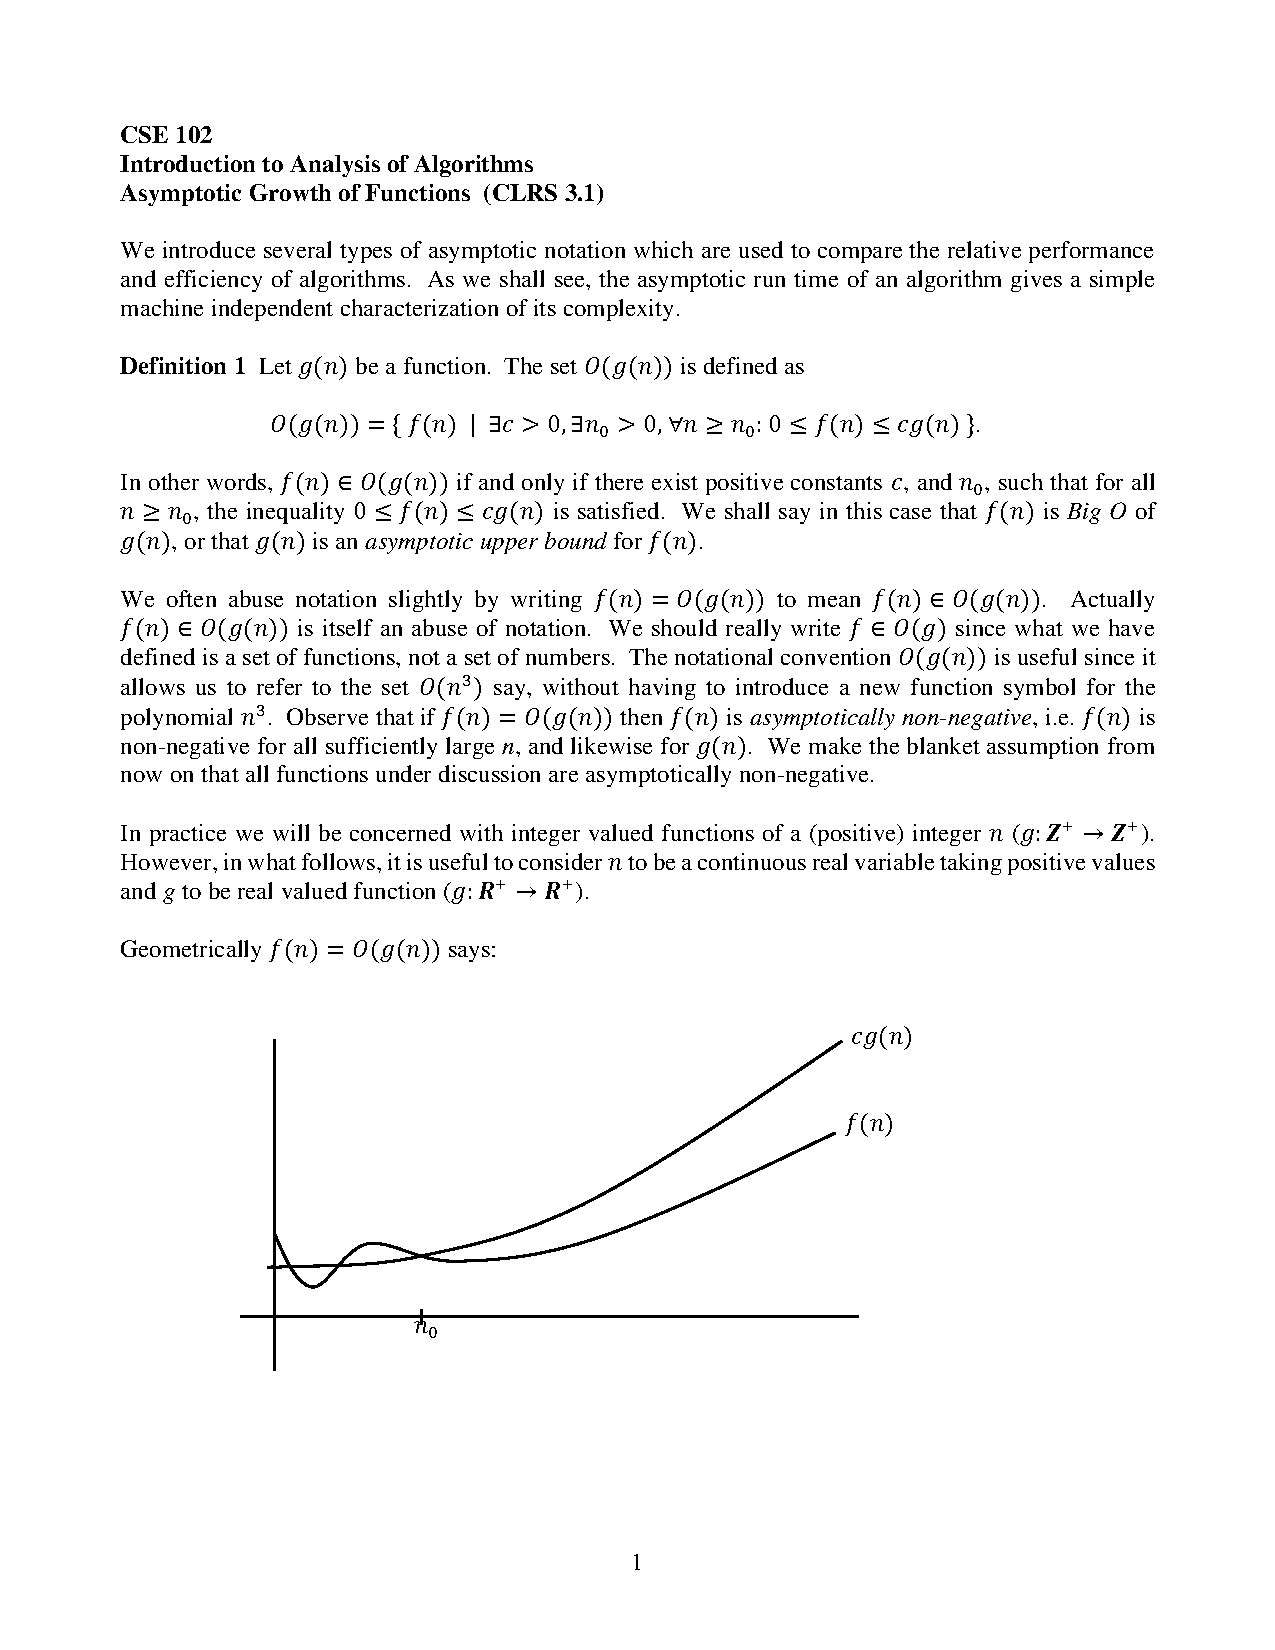
\includepdf[pages=1-9]{Handouts/AsymptoticGrowth.pdf}
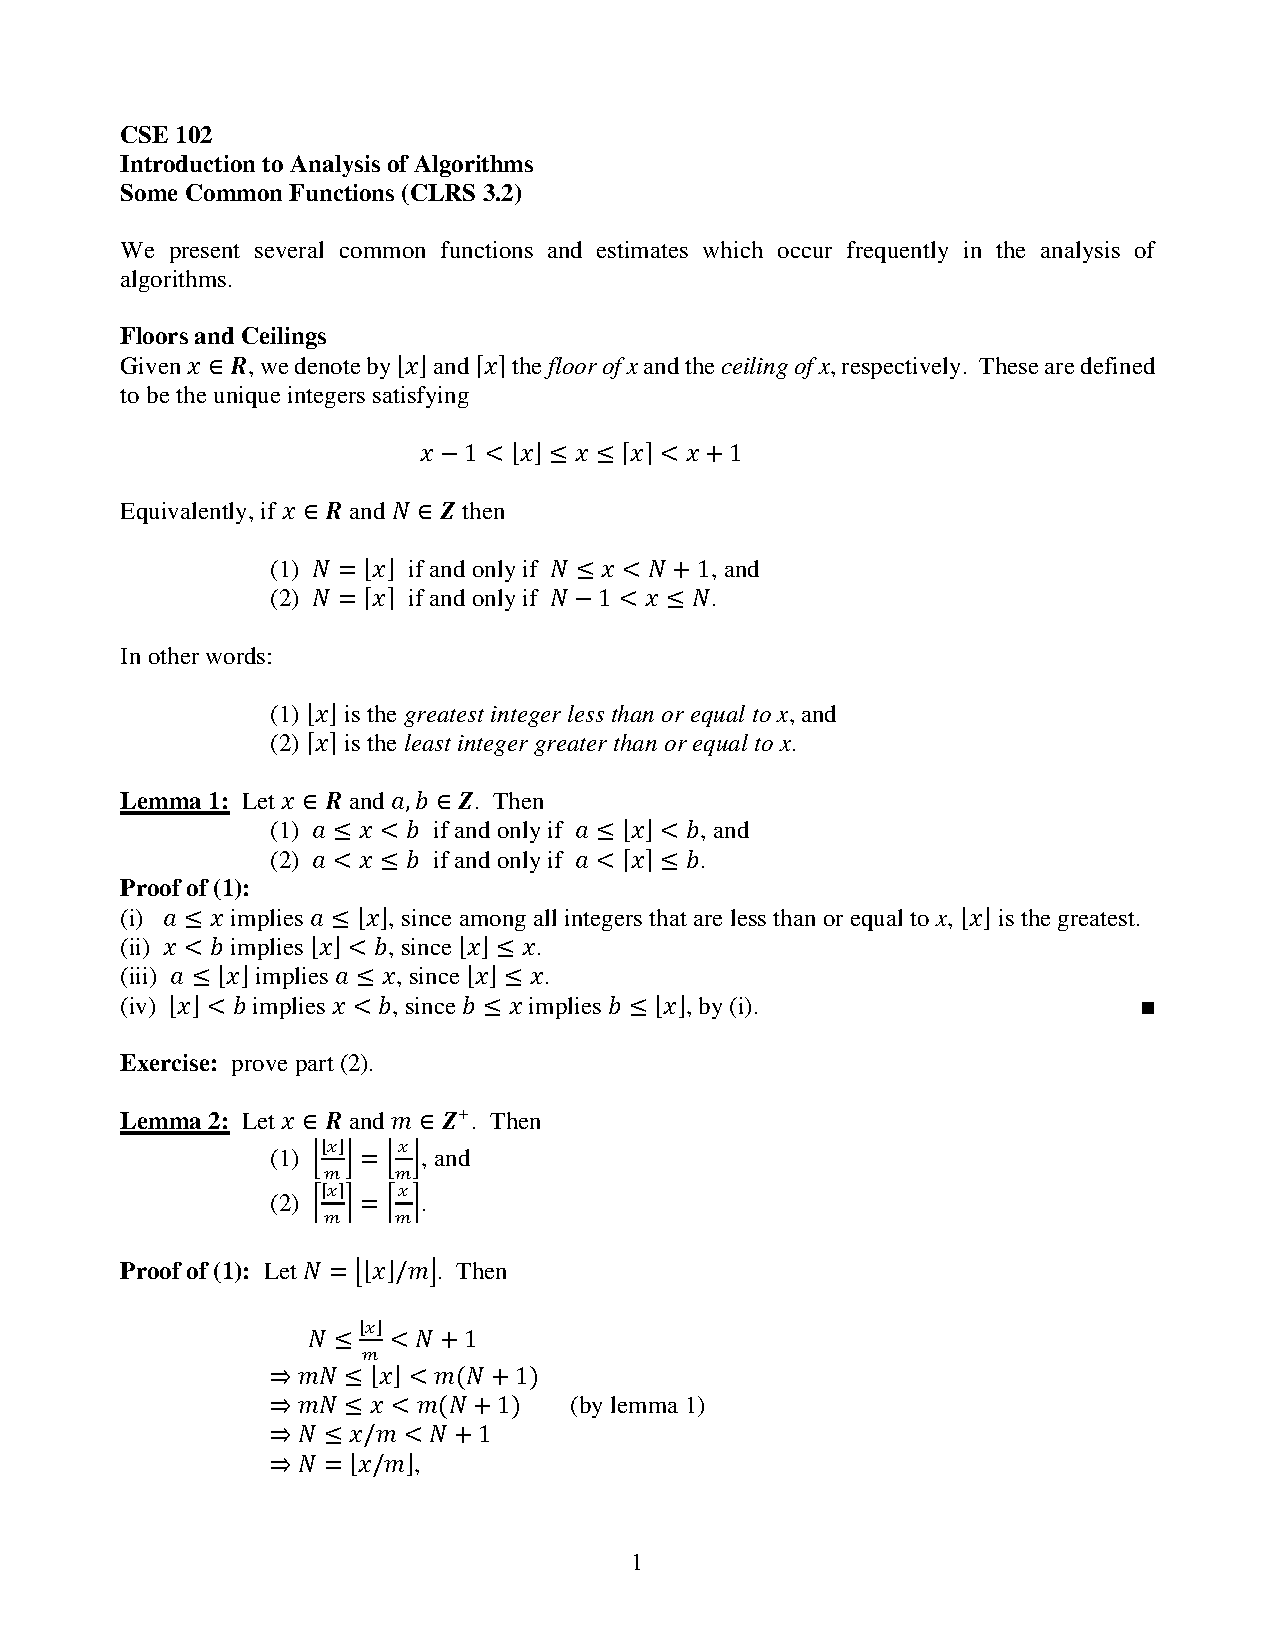
\includepdf[pages=1-3]{Handouts/CommonFunctions.pdf}
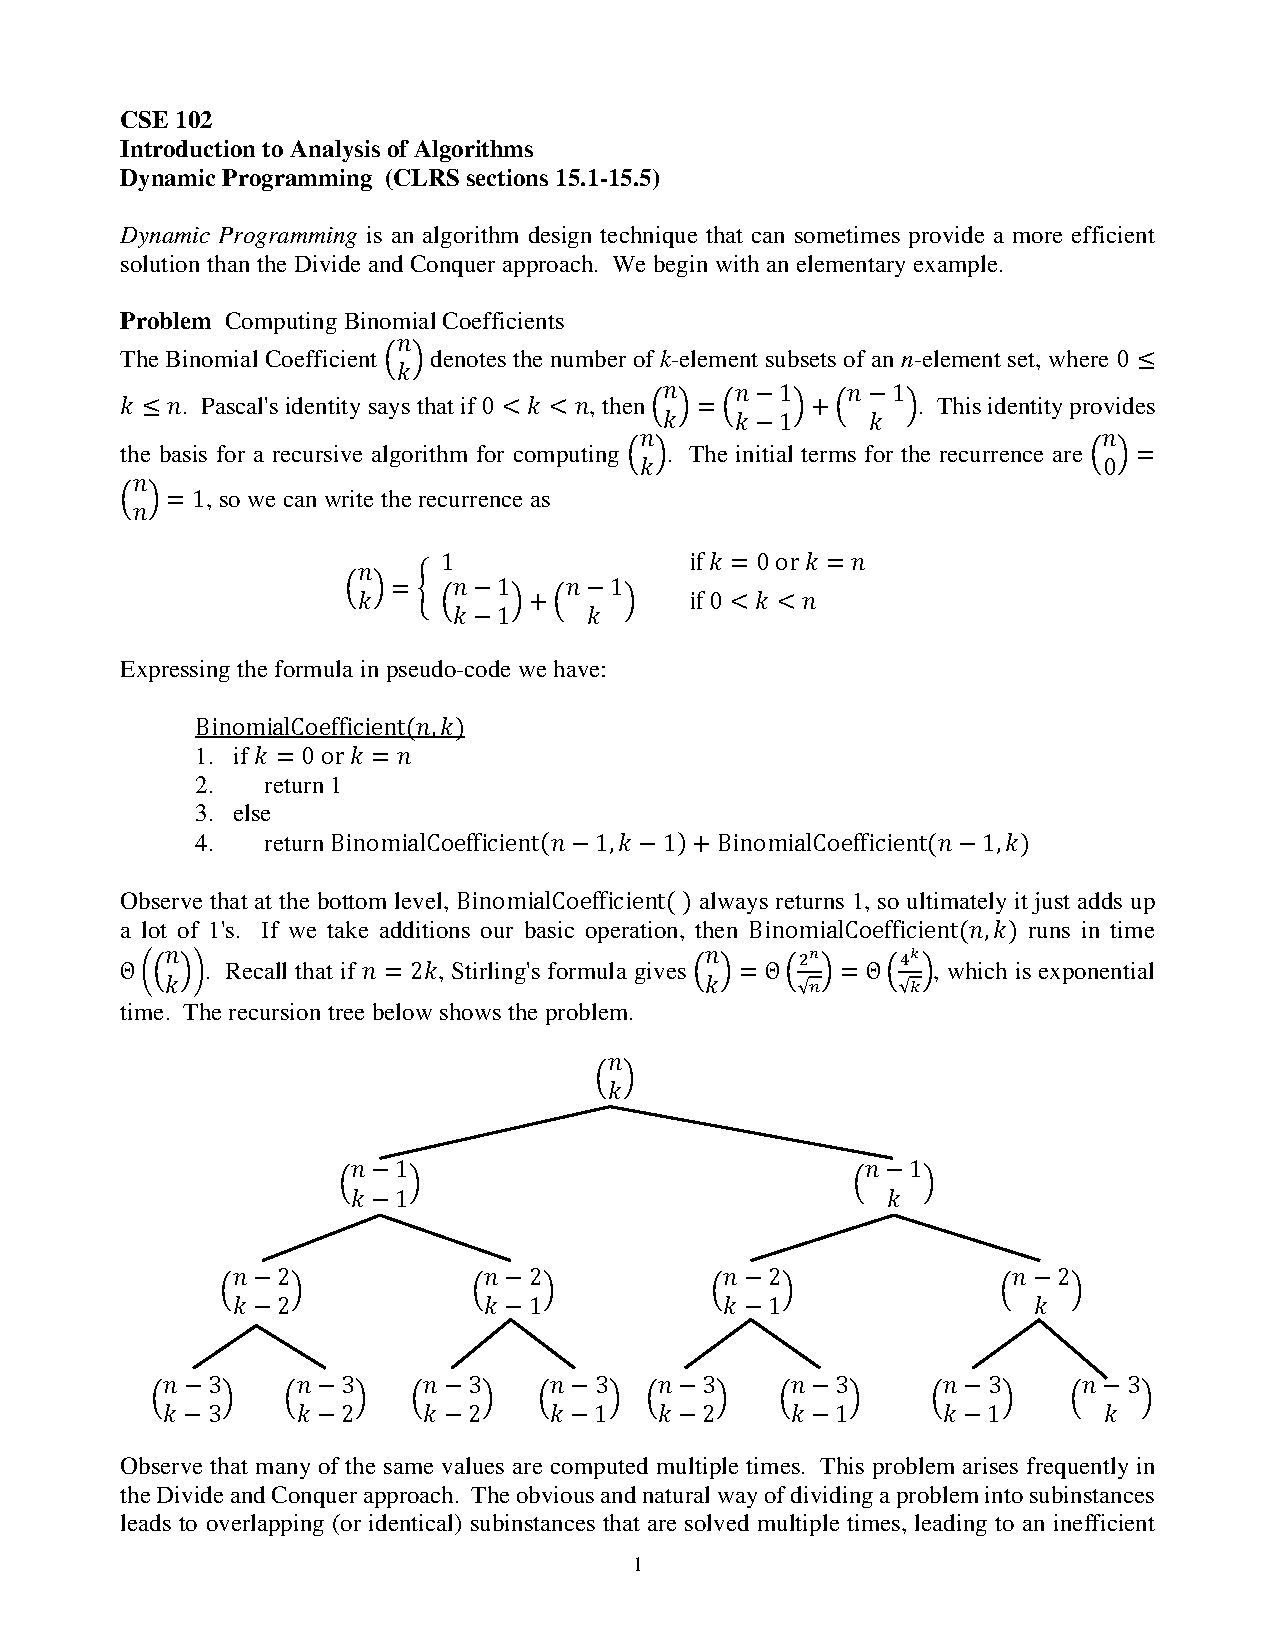
\includepdf[pages=1-11]{Handouts/DynamicProgramming.pdf}
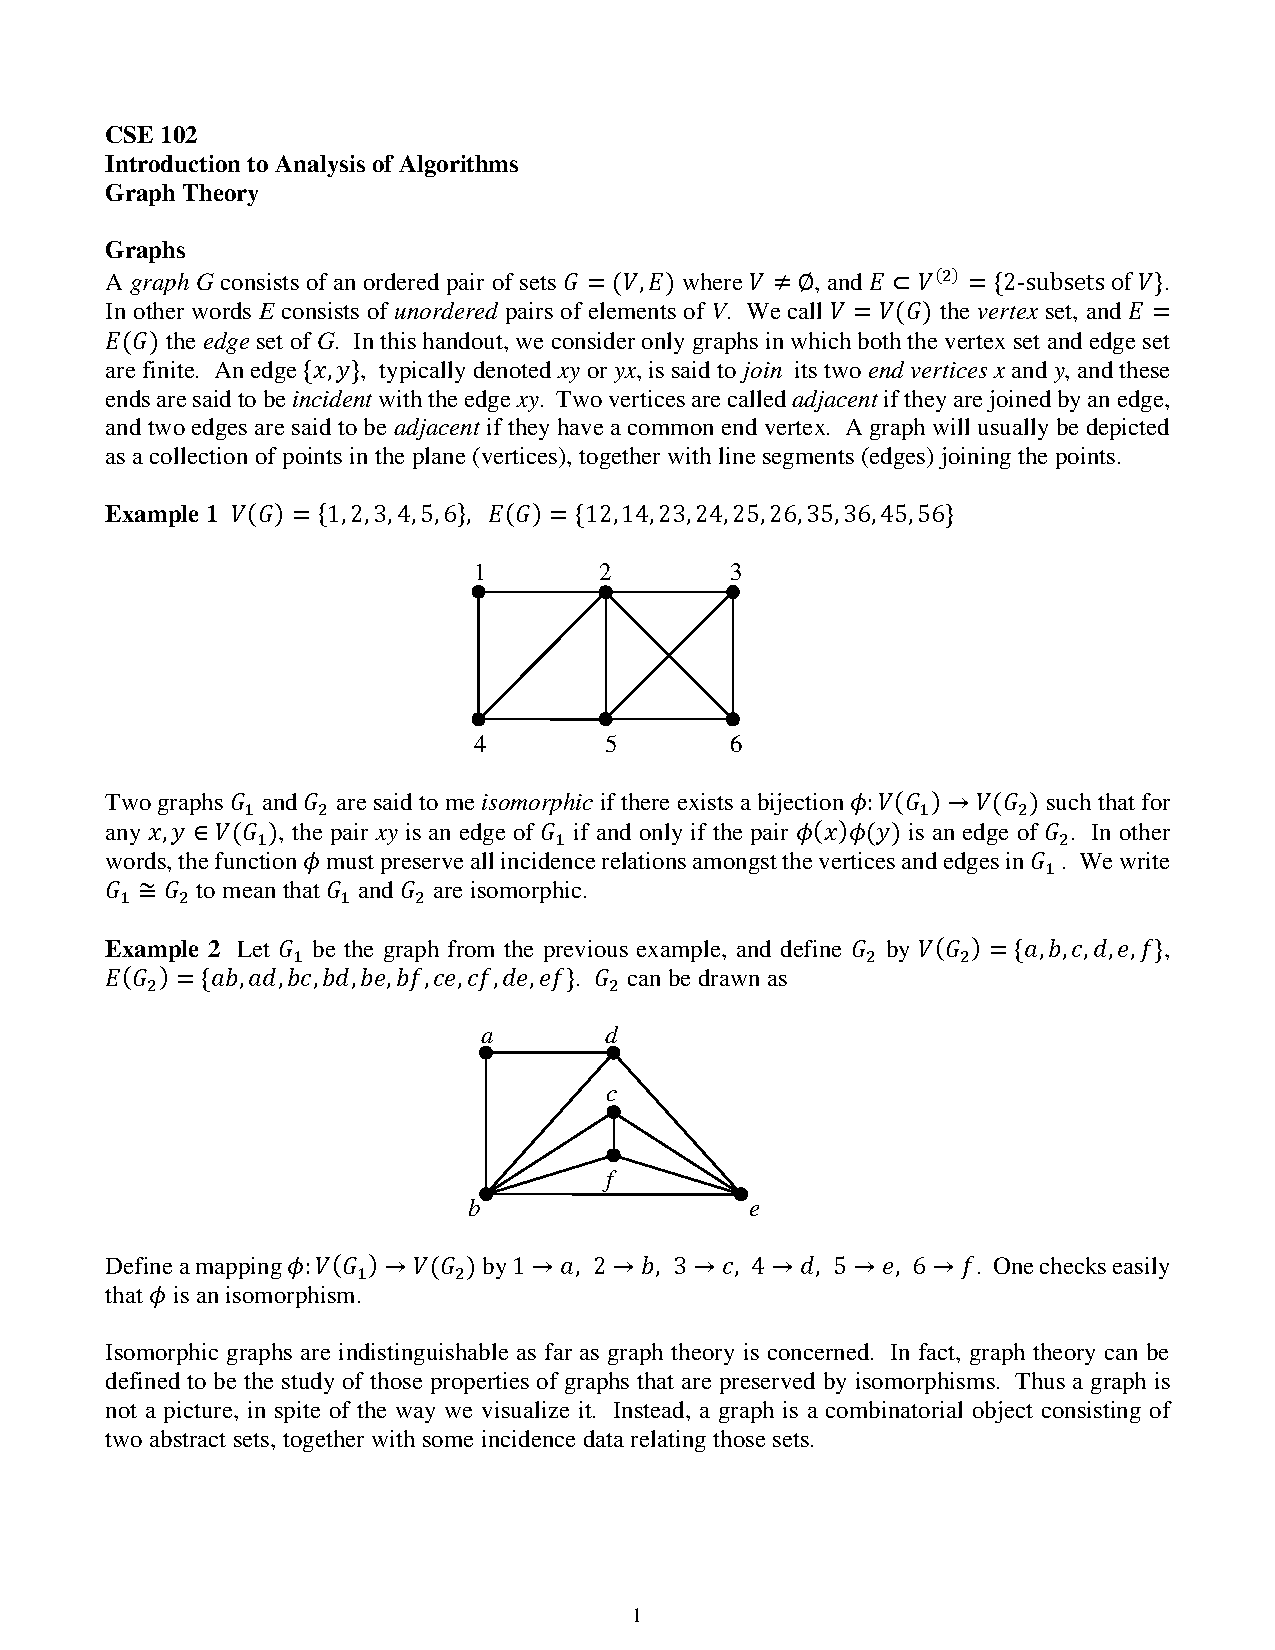
\includepdf[pages=1-11]{Handouts/GraphTheory.pdf}
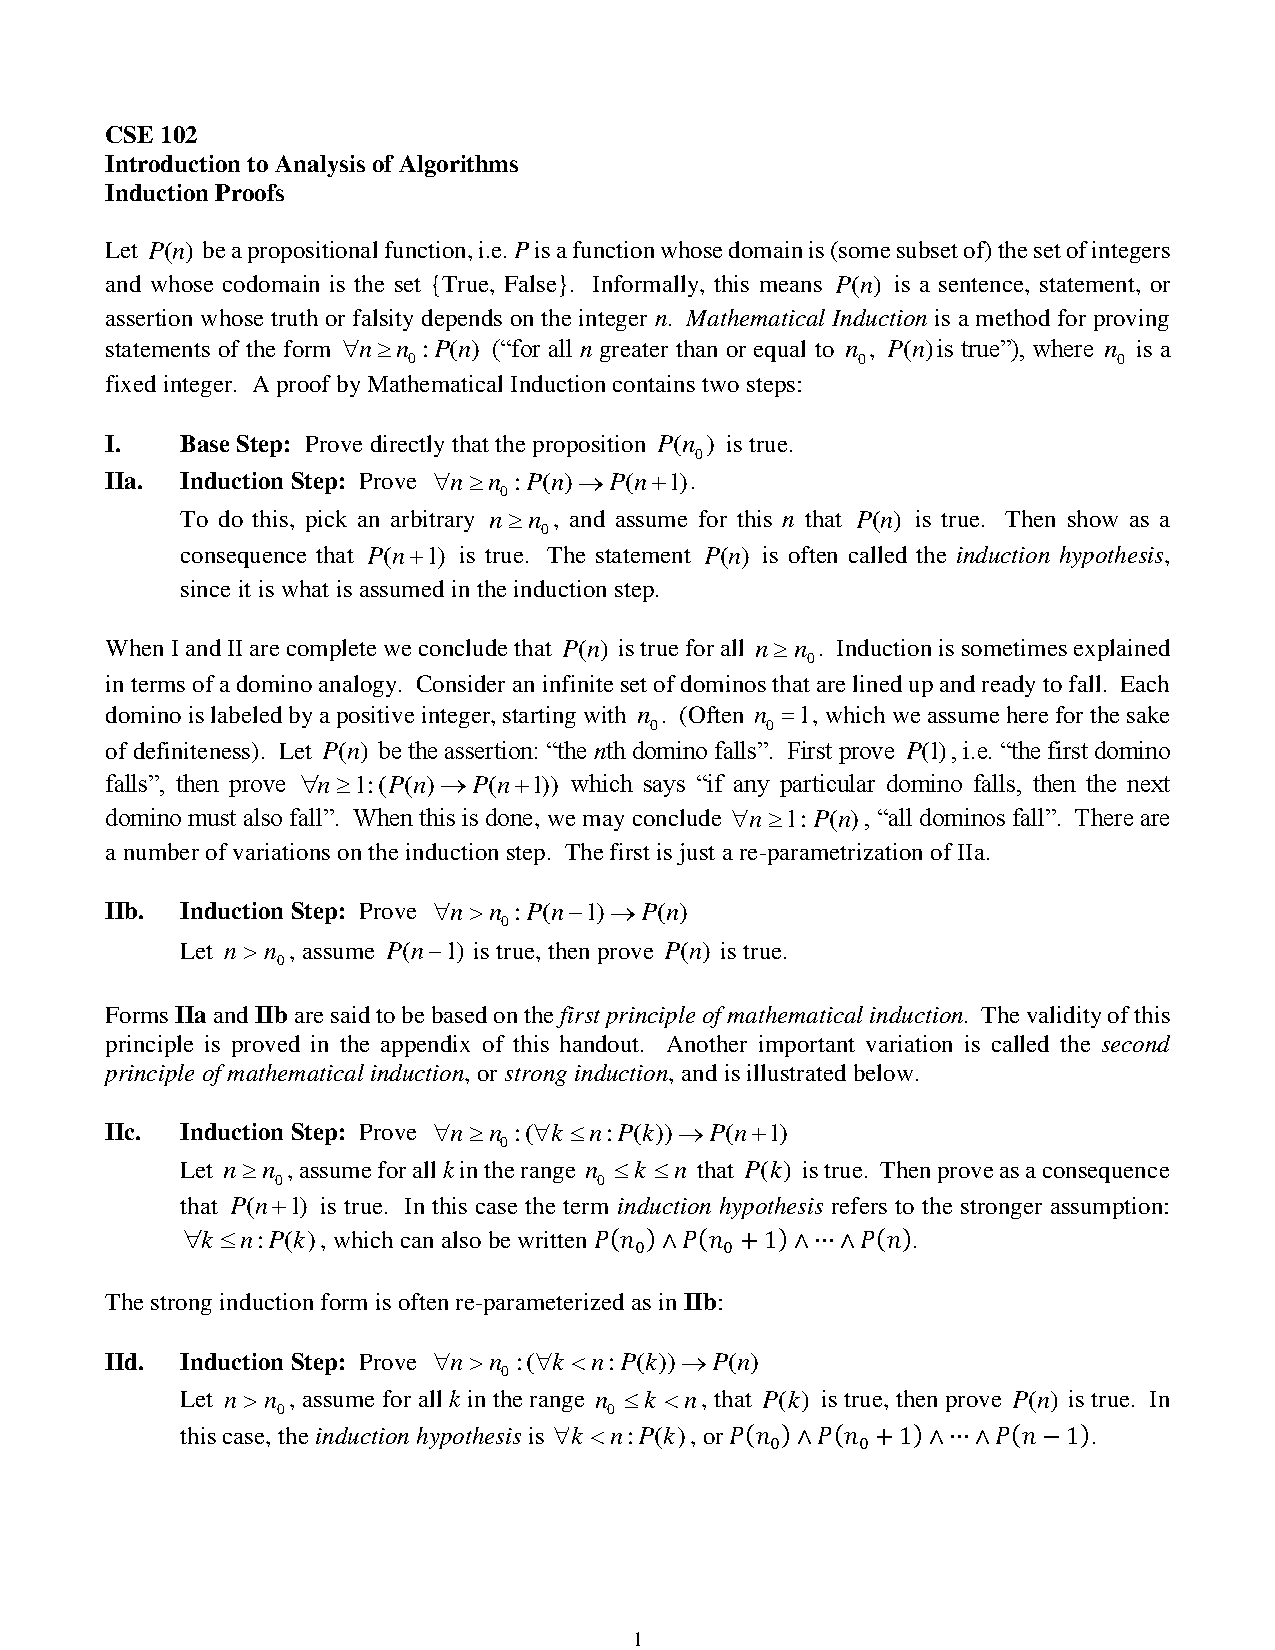
\includepdf[pages=1-11]{Handouts/InductionProofs.pdf}
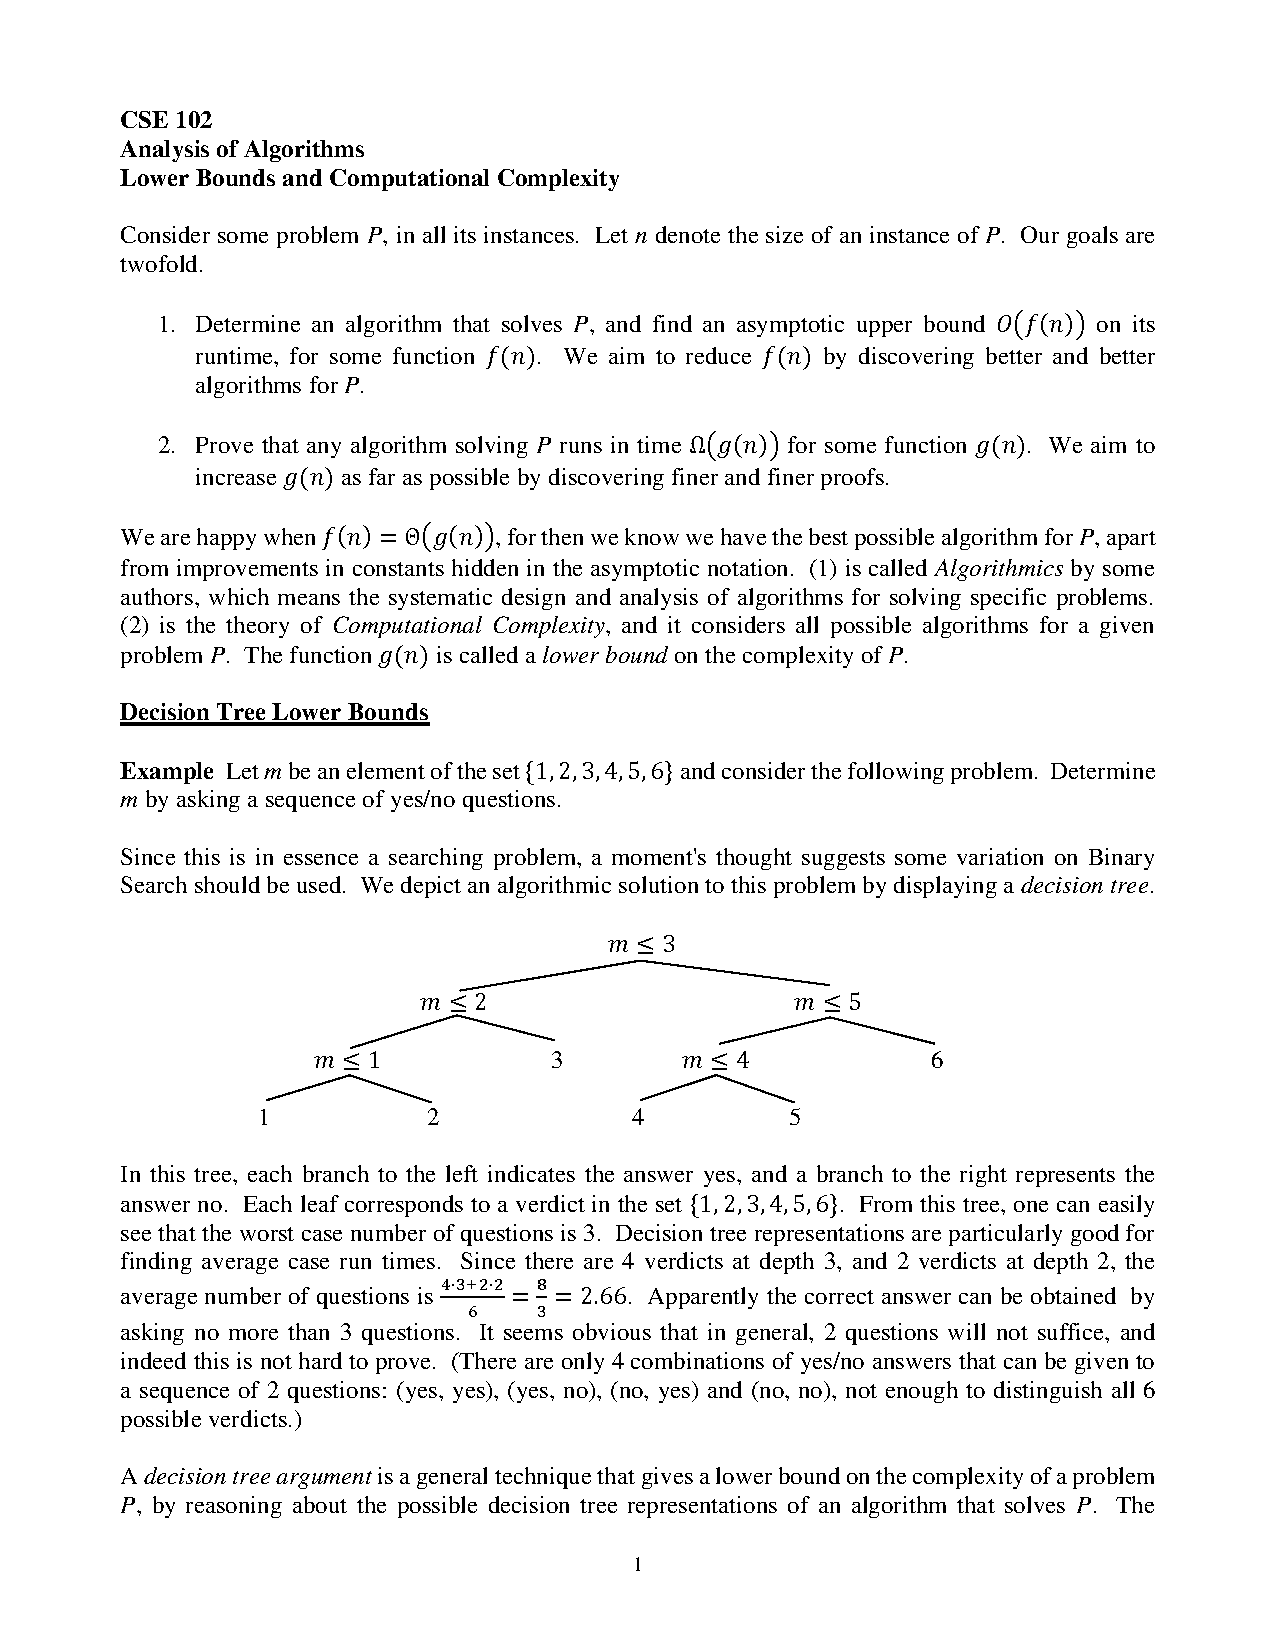
\includepdf[pages=1-11]{Handouts/LowerBounds.pdf}
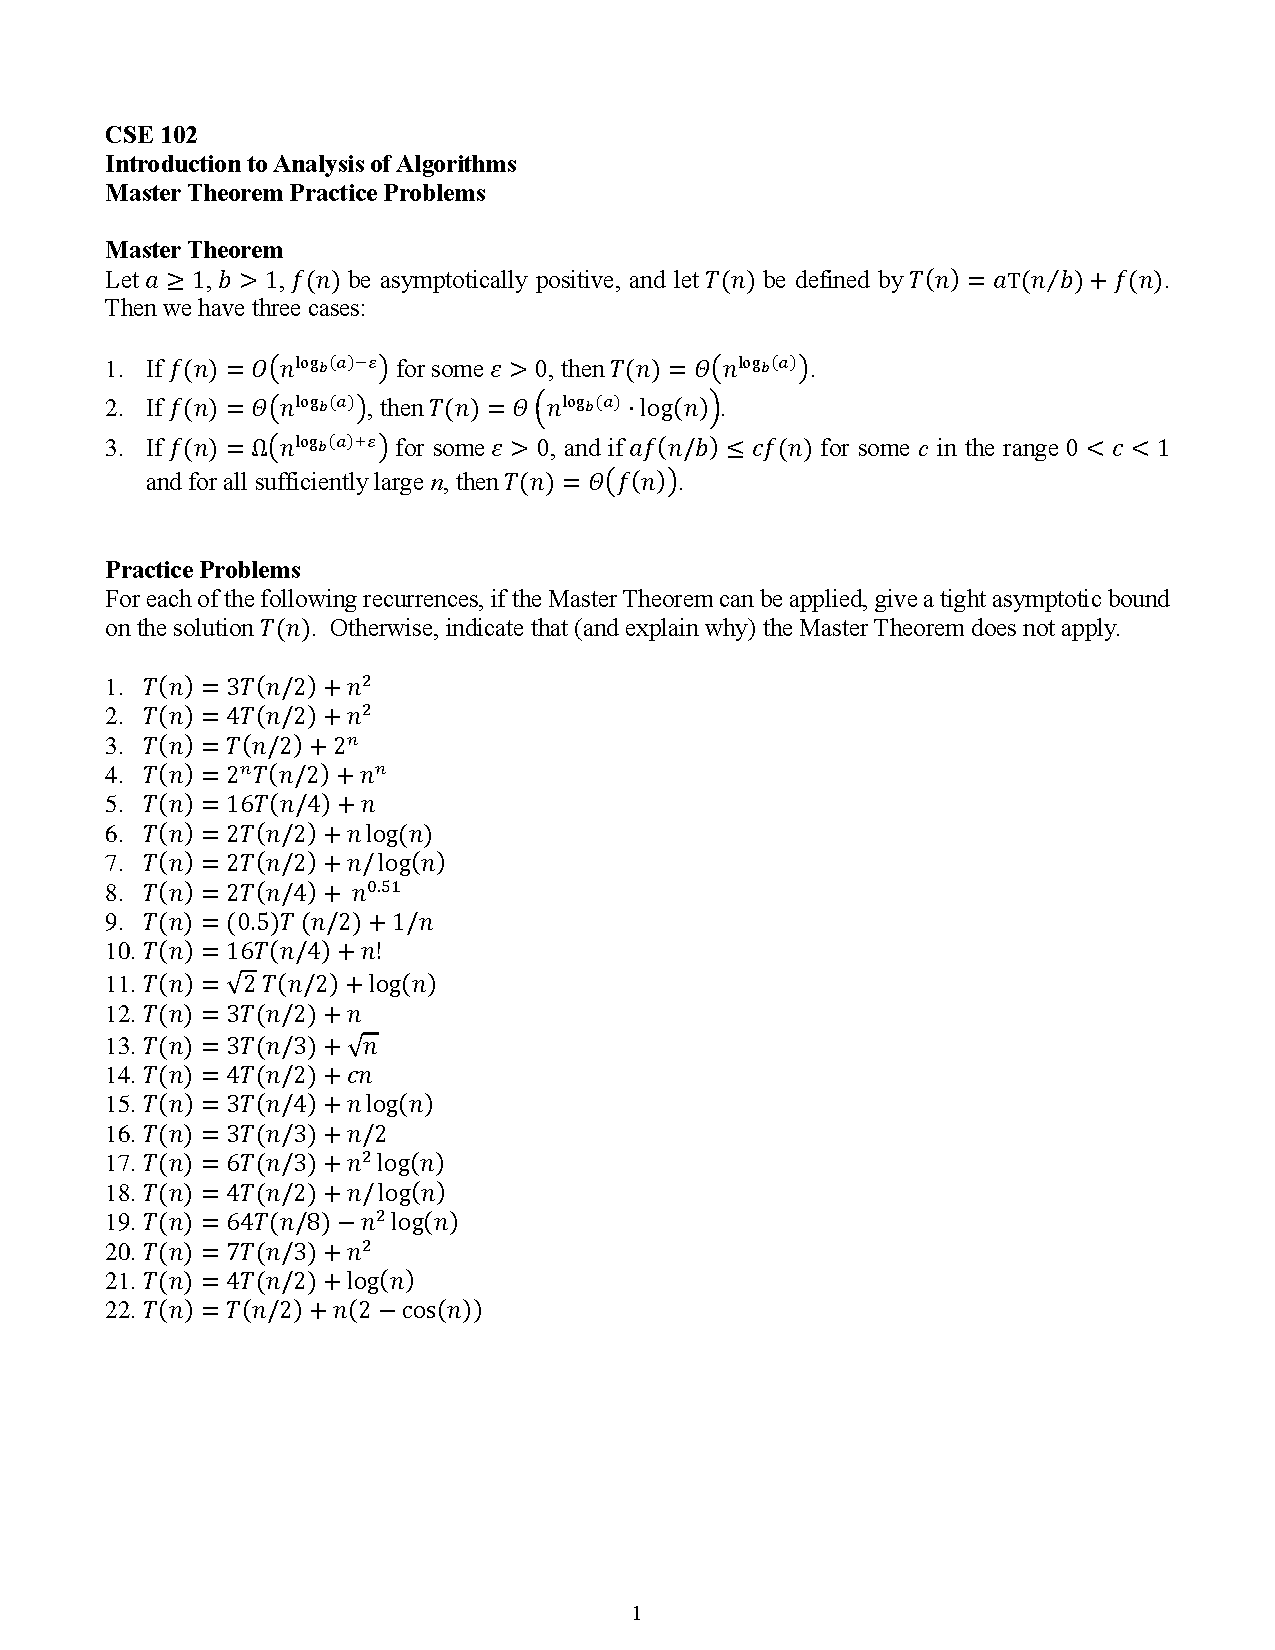
\includepdf[pages=1-2]{Handouts/MasterTheoremPracticeProblems.pdf}
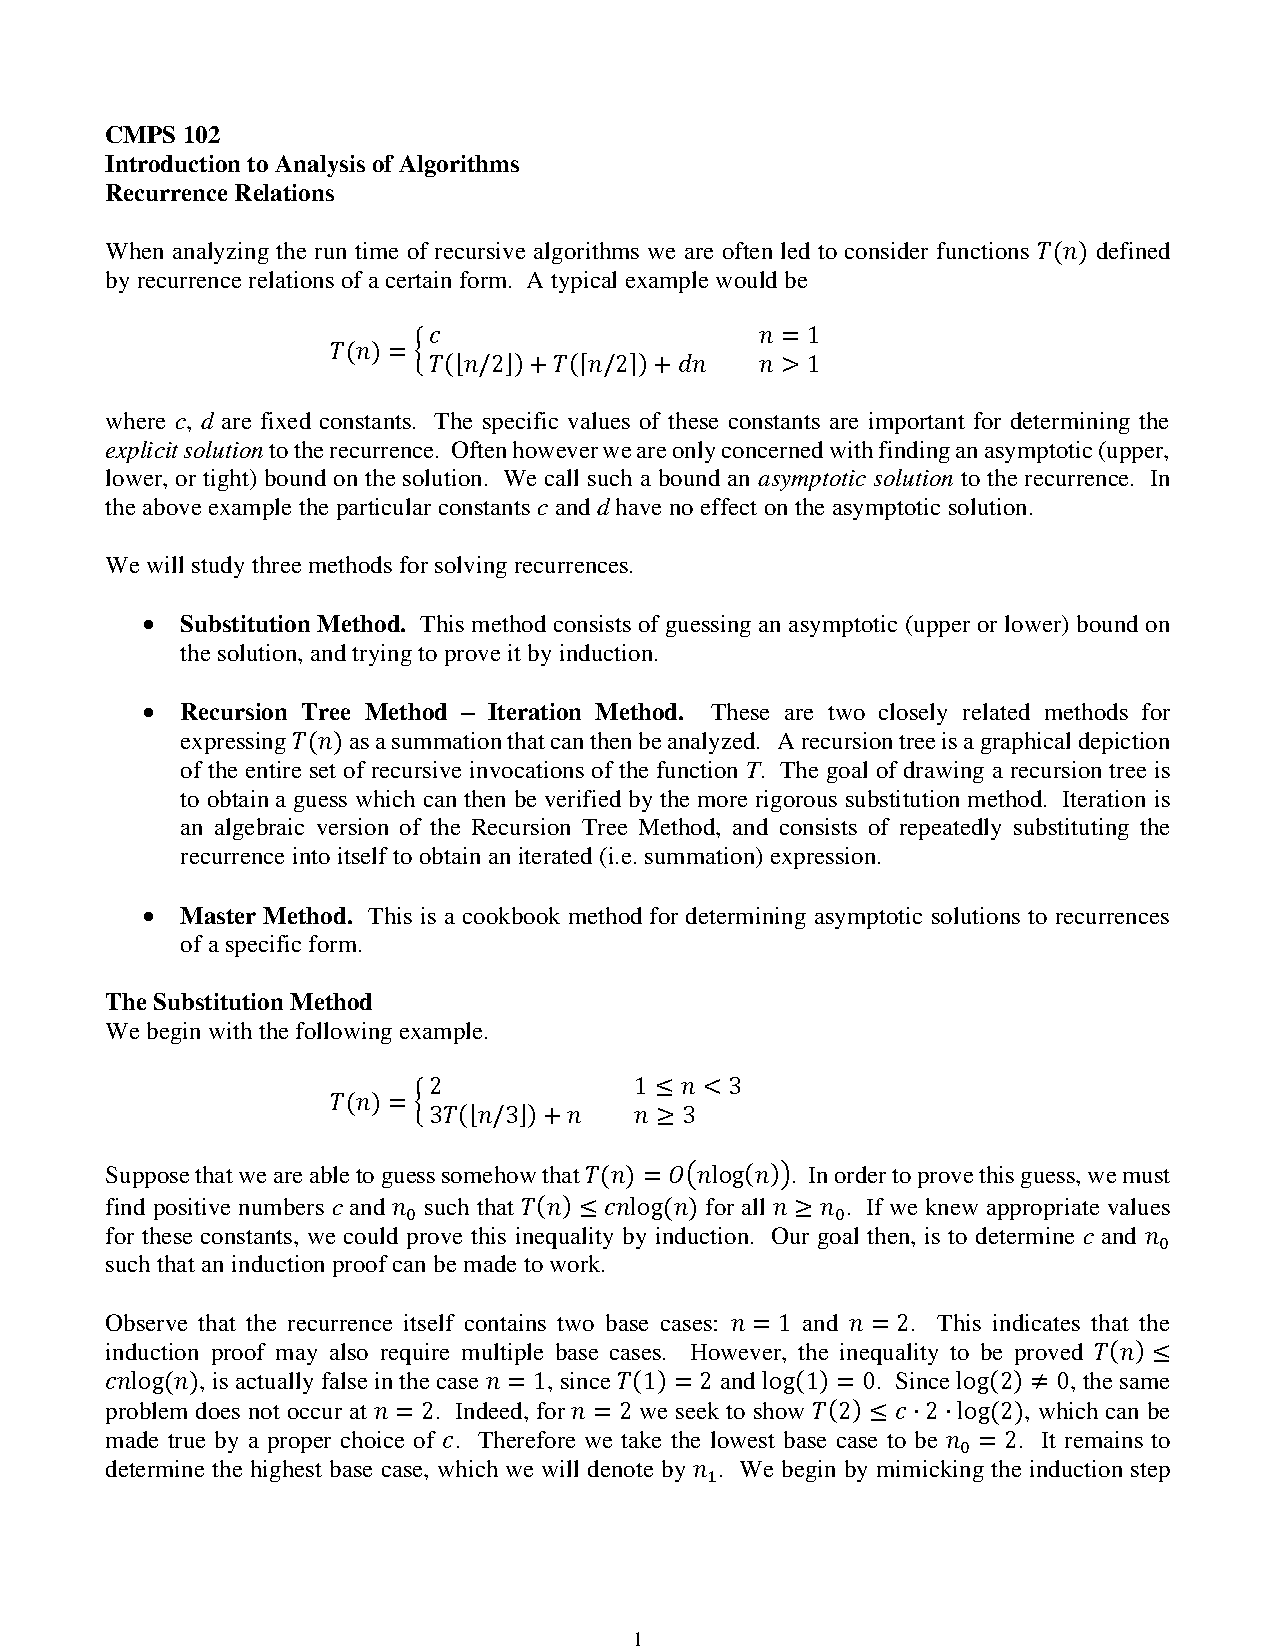
\includepdf[pages=1-12]{Handouts/Recurrence.pdf}
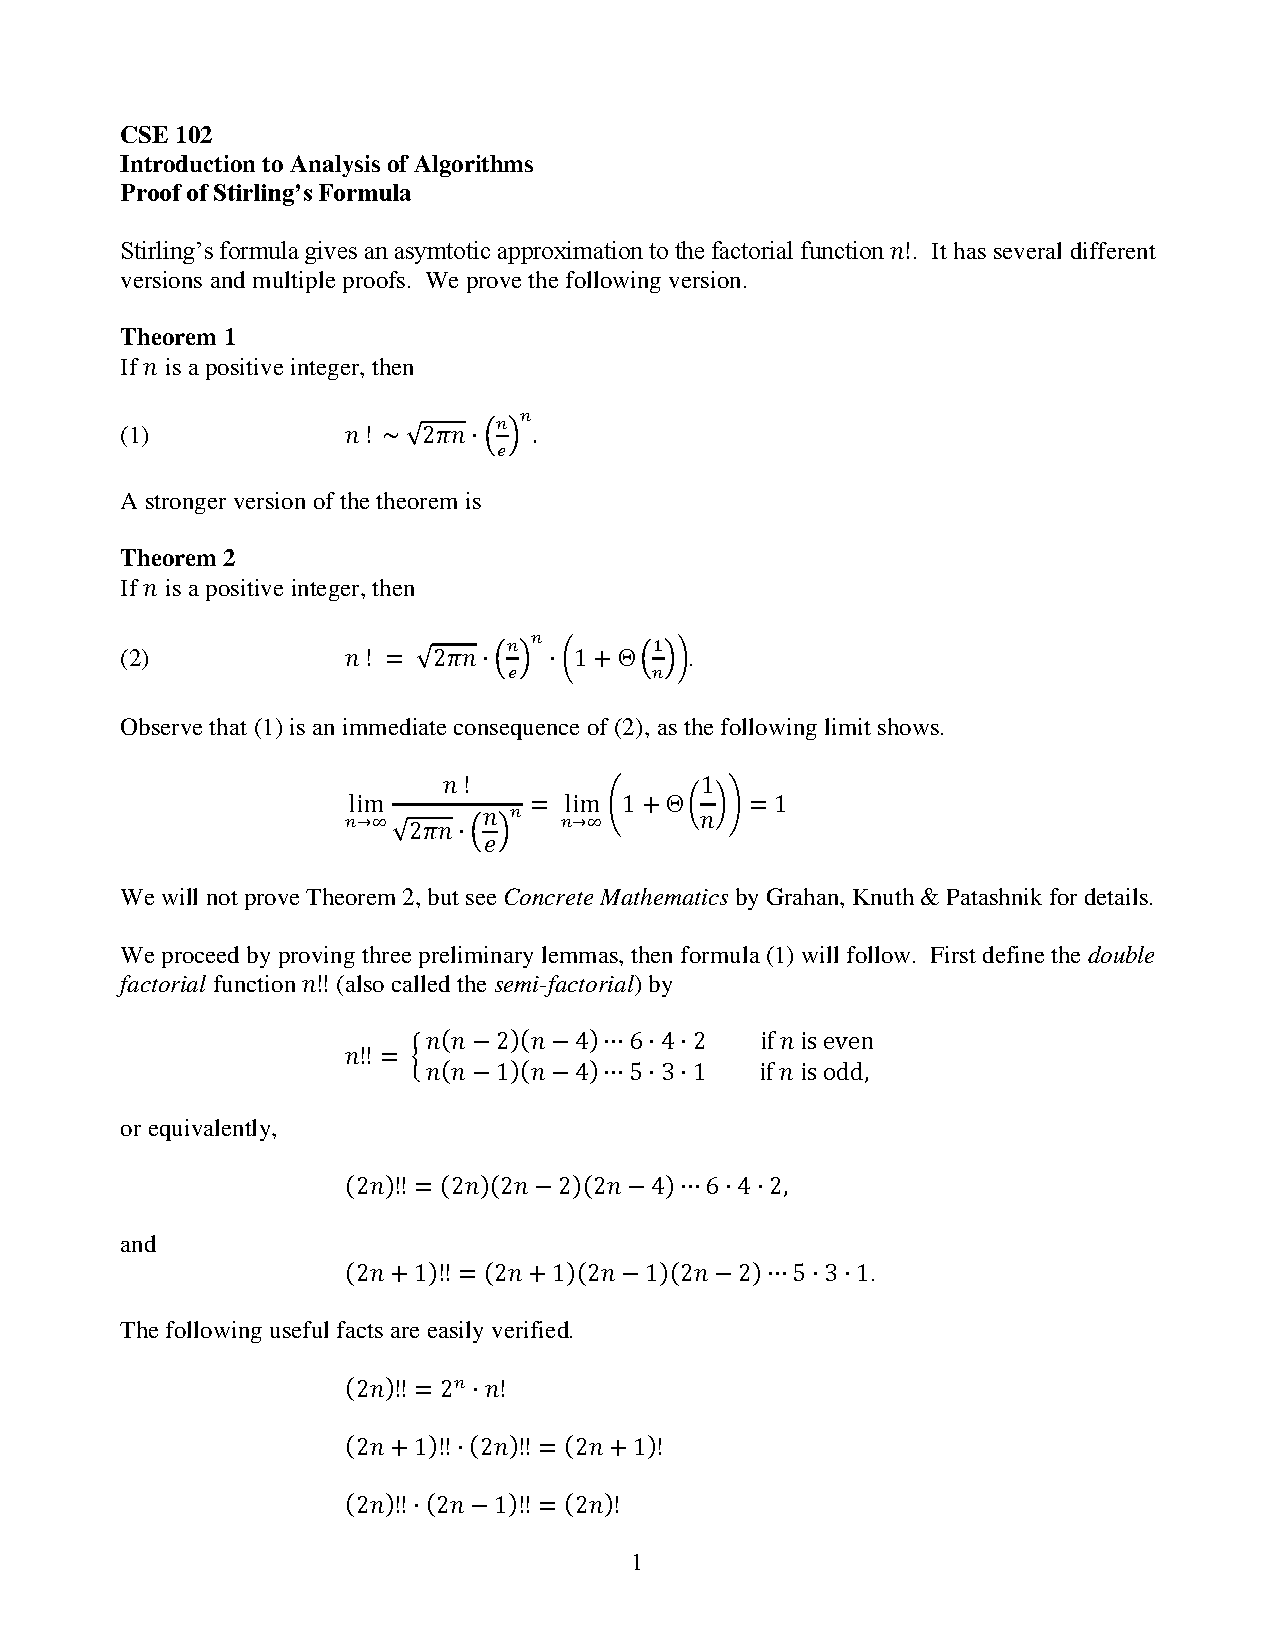
\includepdf[pages=1-6]{Handouts/StirlingFormula.pdf}

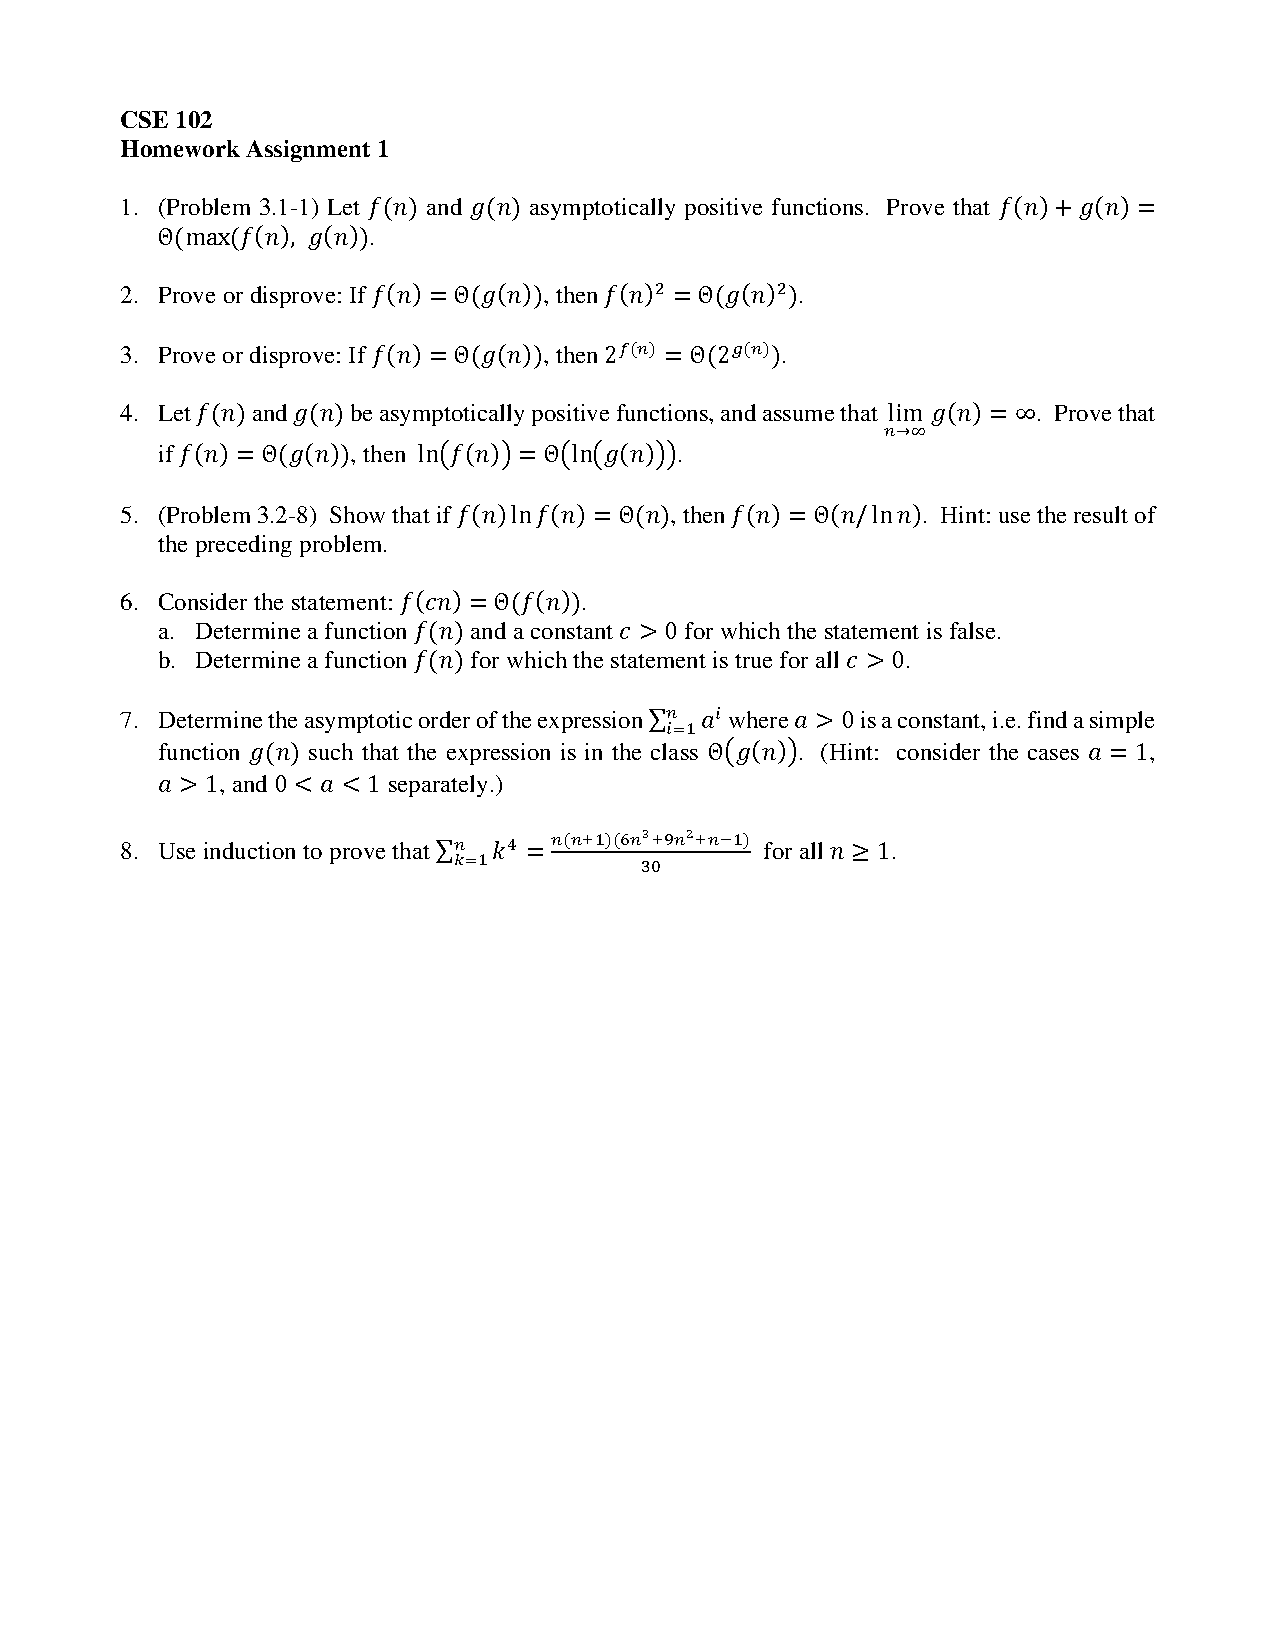
\includepdf[pages=1-1]{homework/hw1.pdf}
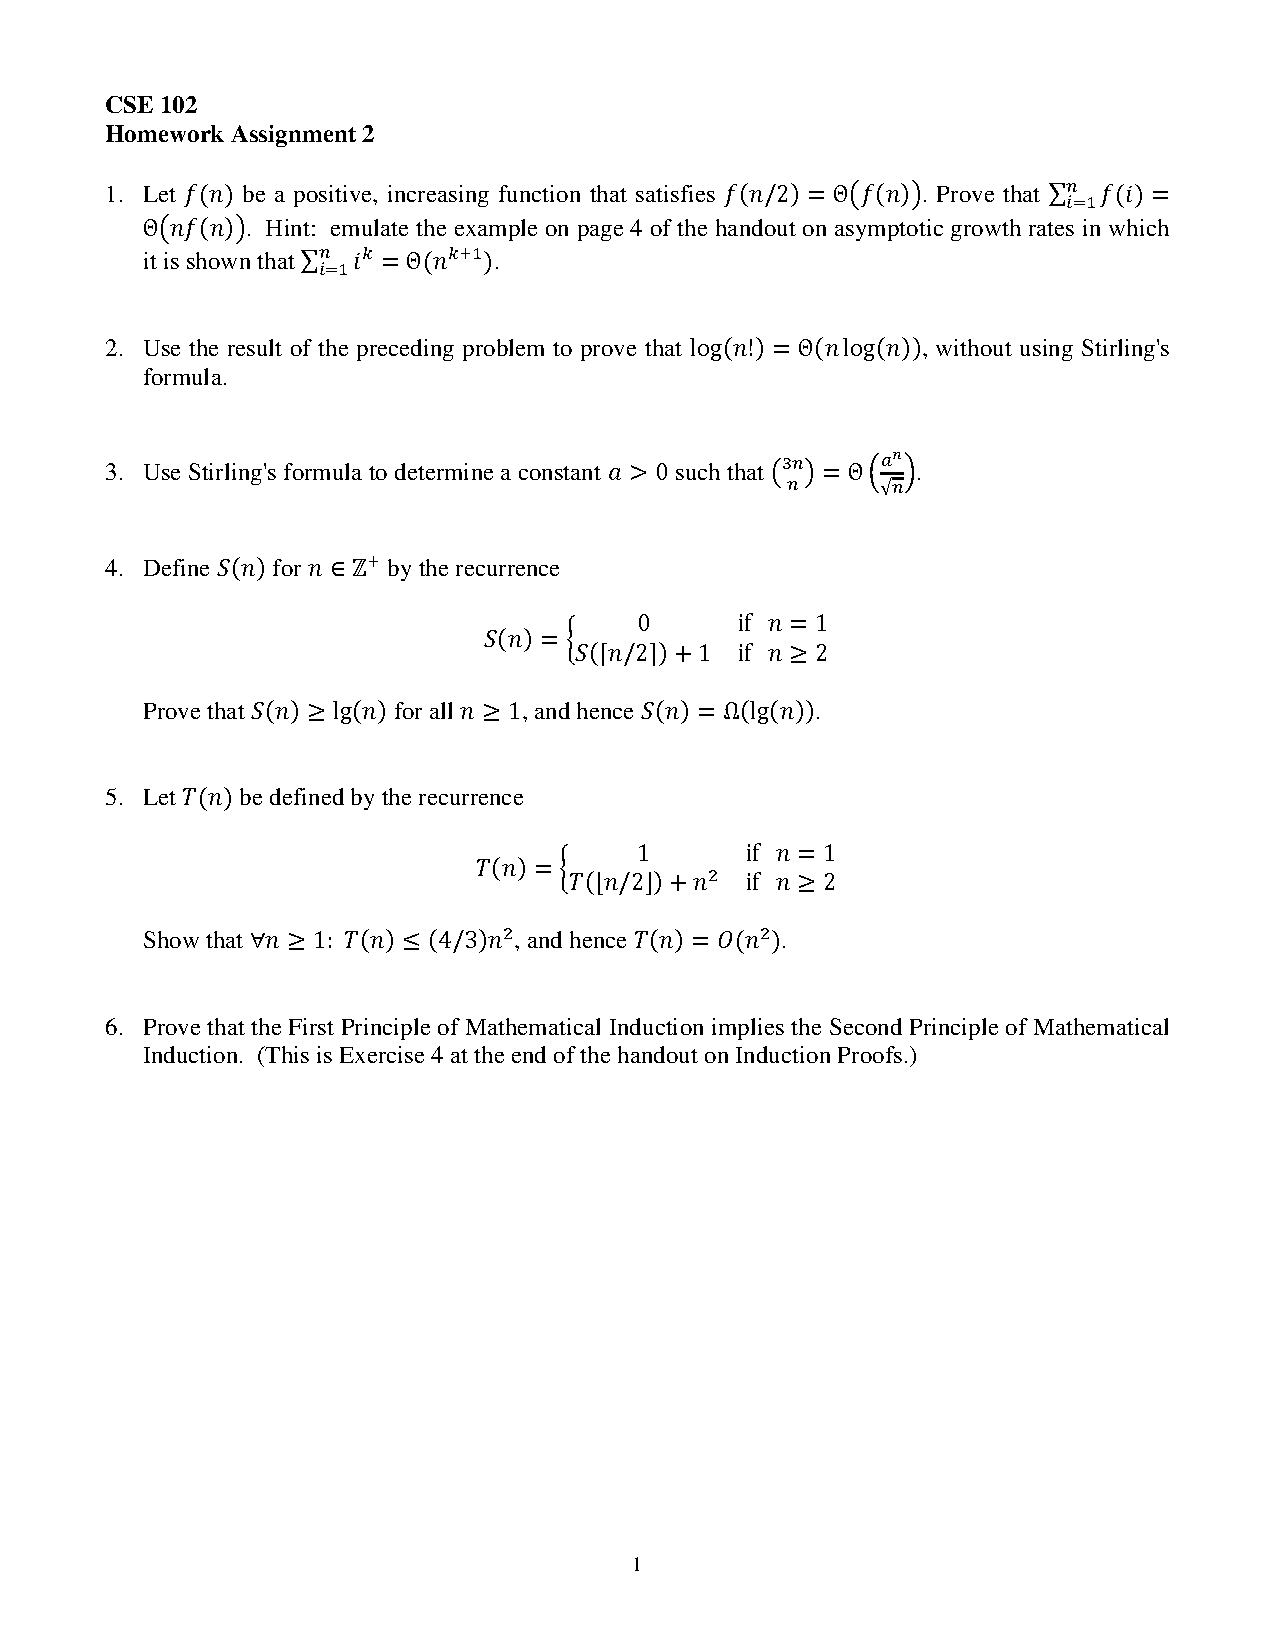
\includepdf[pages=1-1]{homework/hw2.pdf}
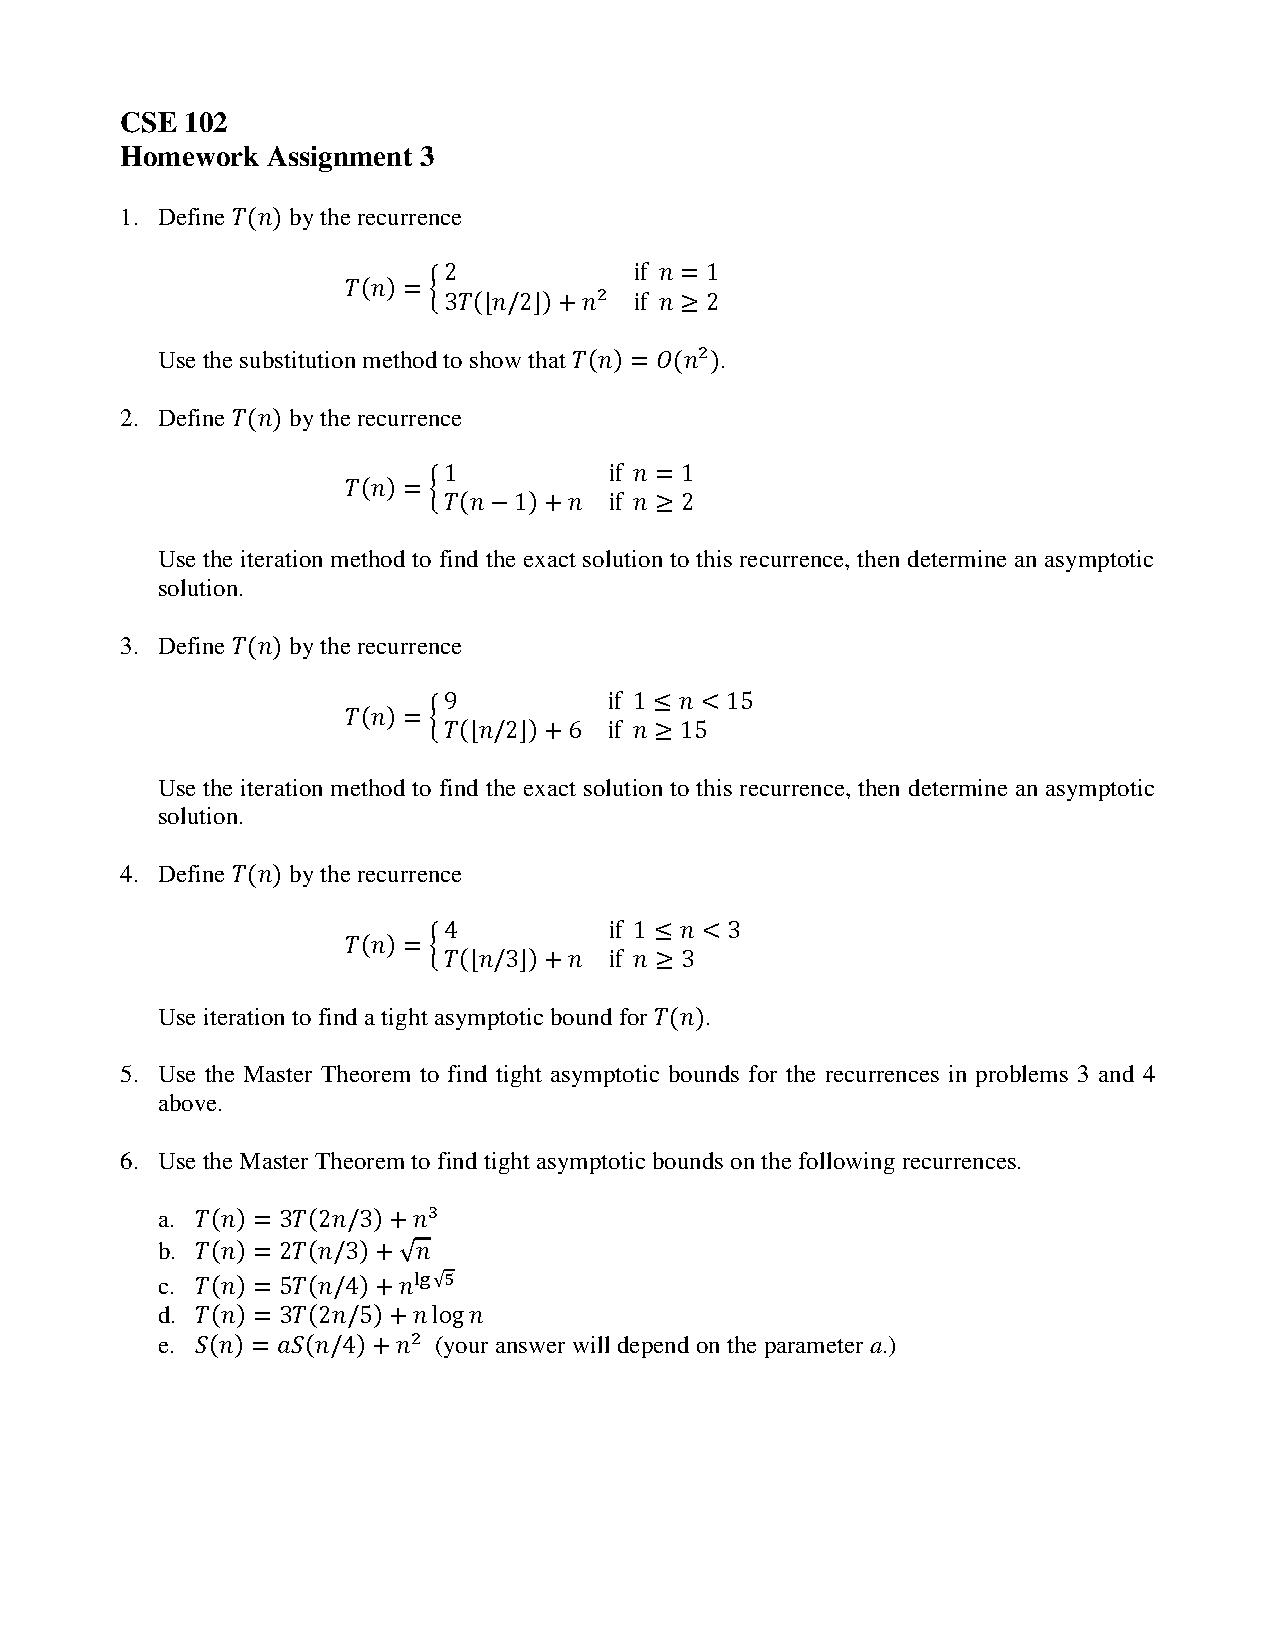
\includepdf[pages=1-1]{homework/hw3.pdf}
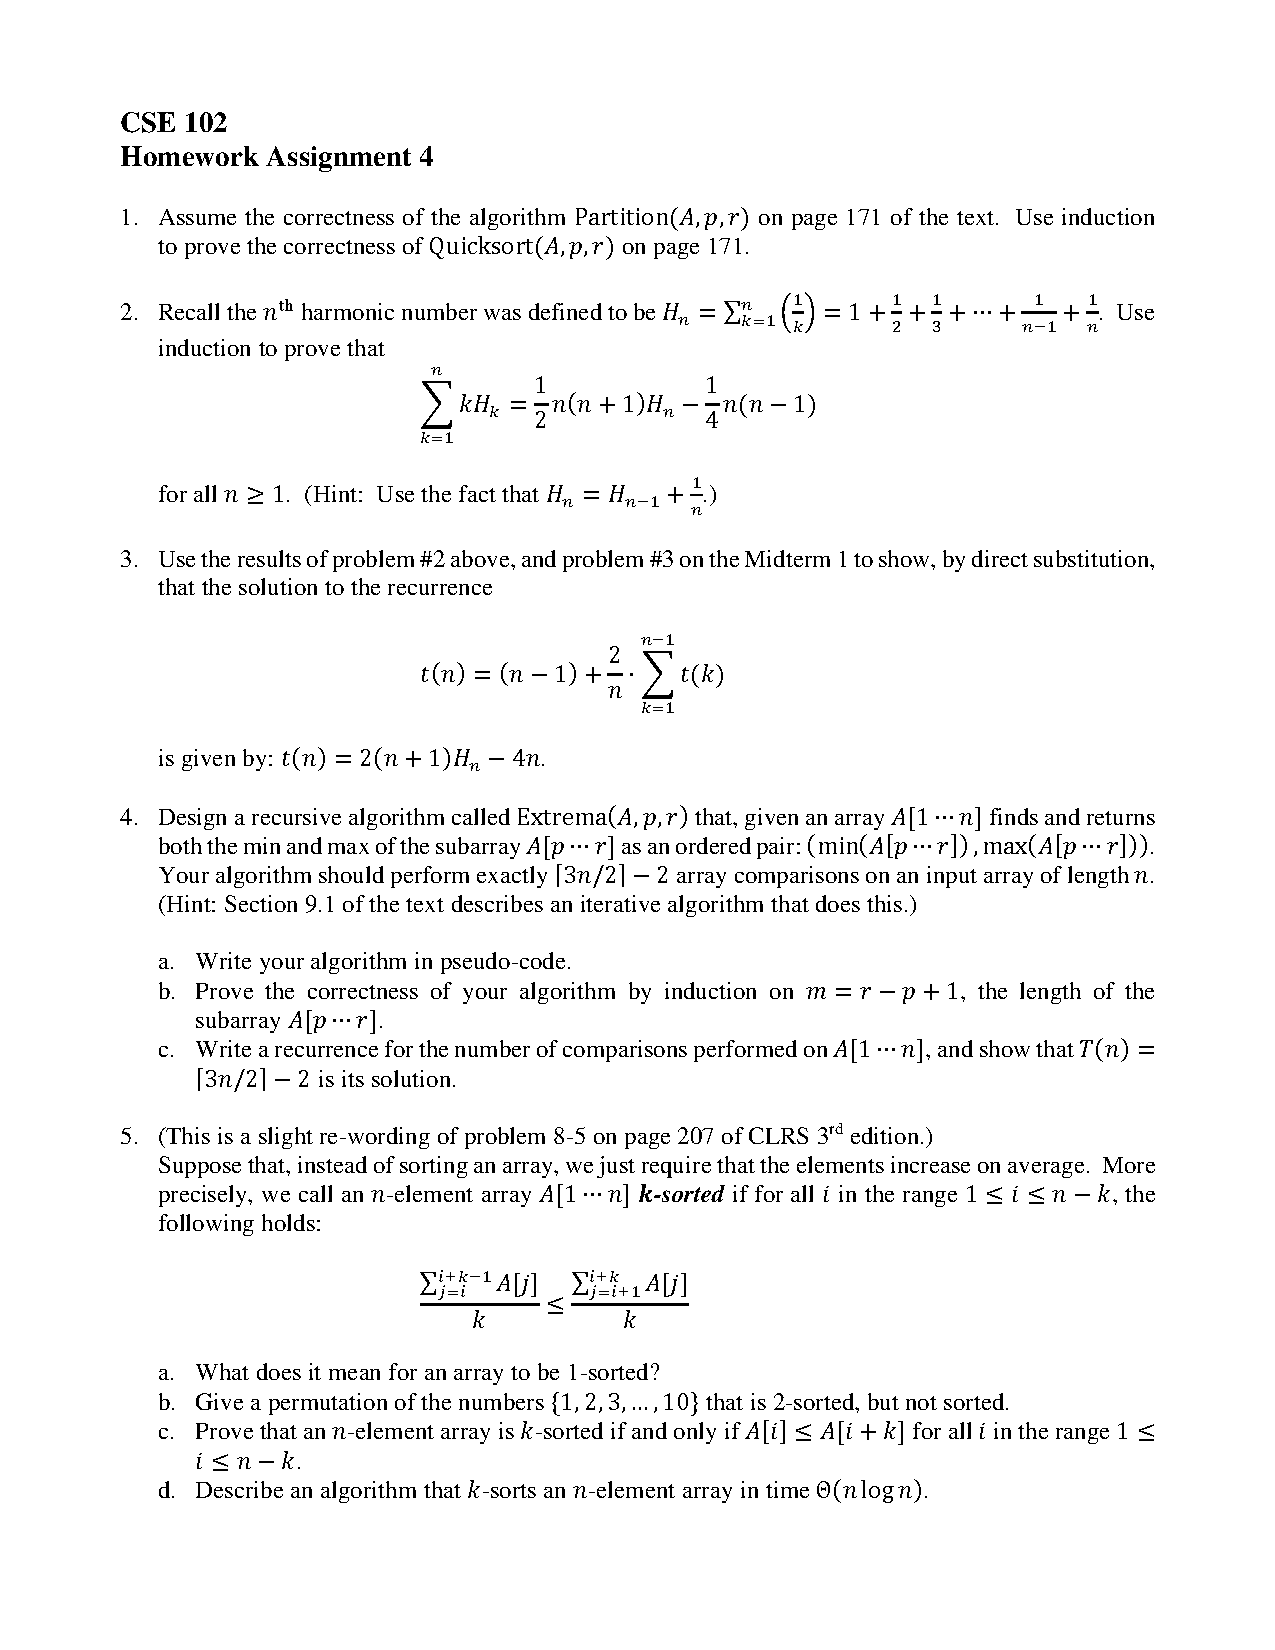
\includepdf[pages=1-1]{homework/hw4.pdf}
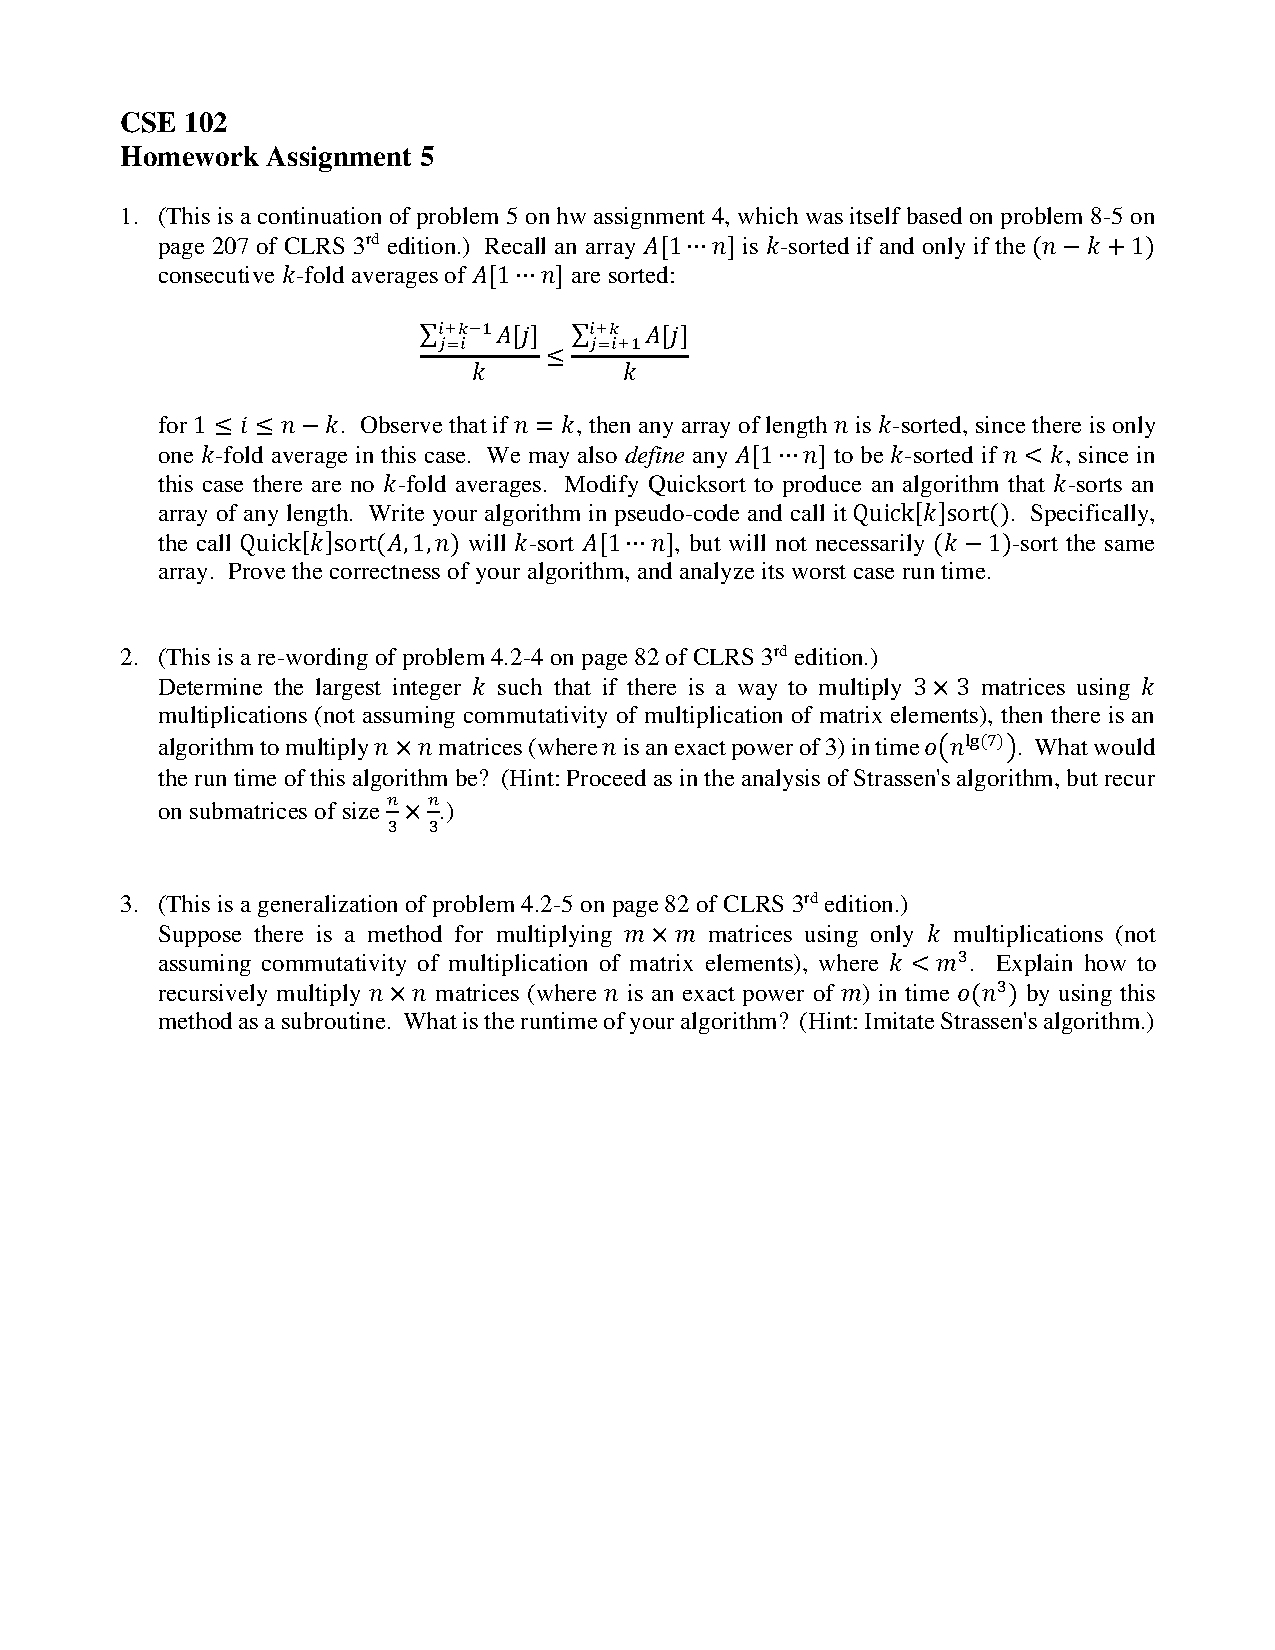
\includepdf[pages=1-2]{homework/hw5.pdf}
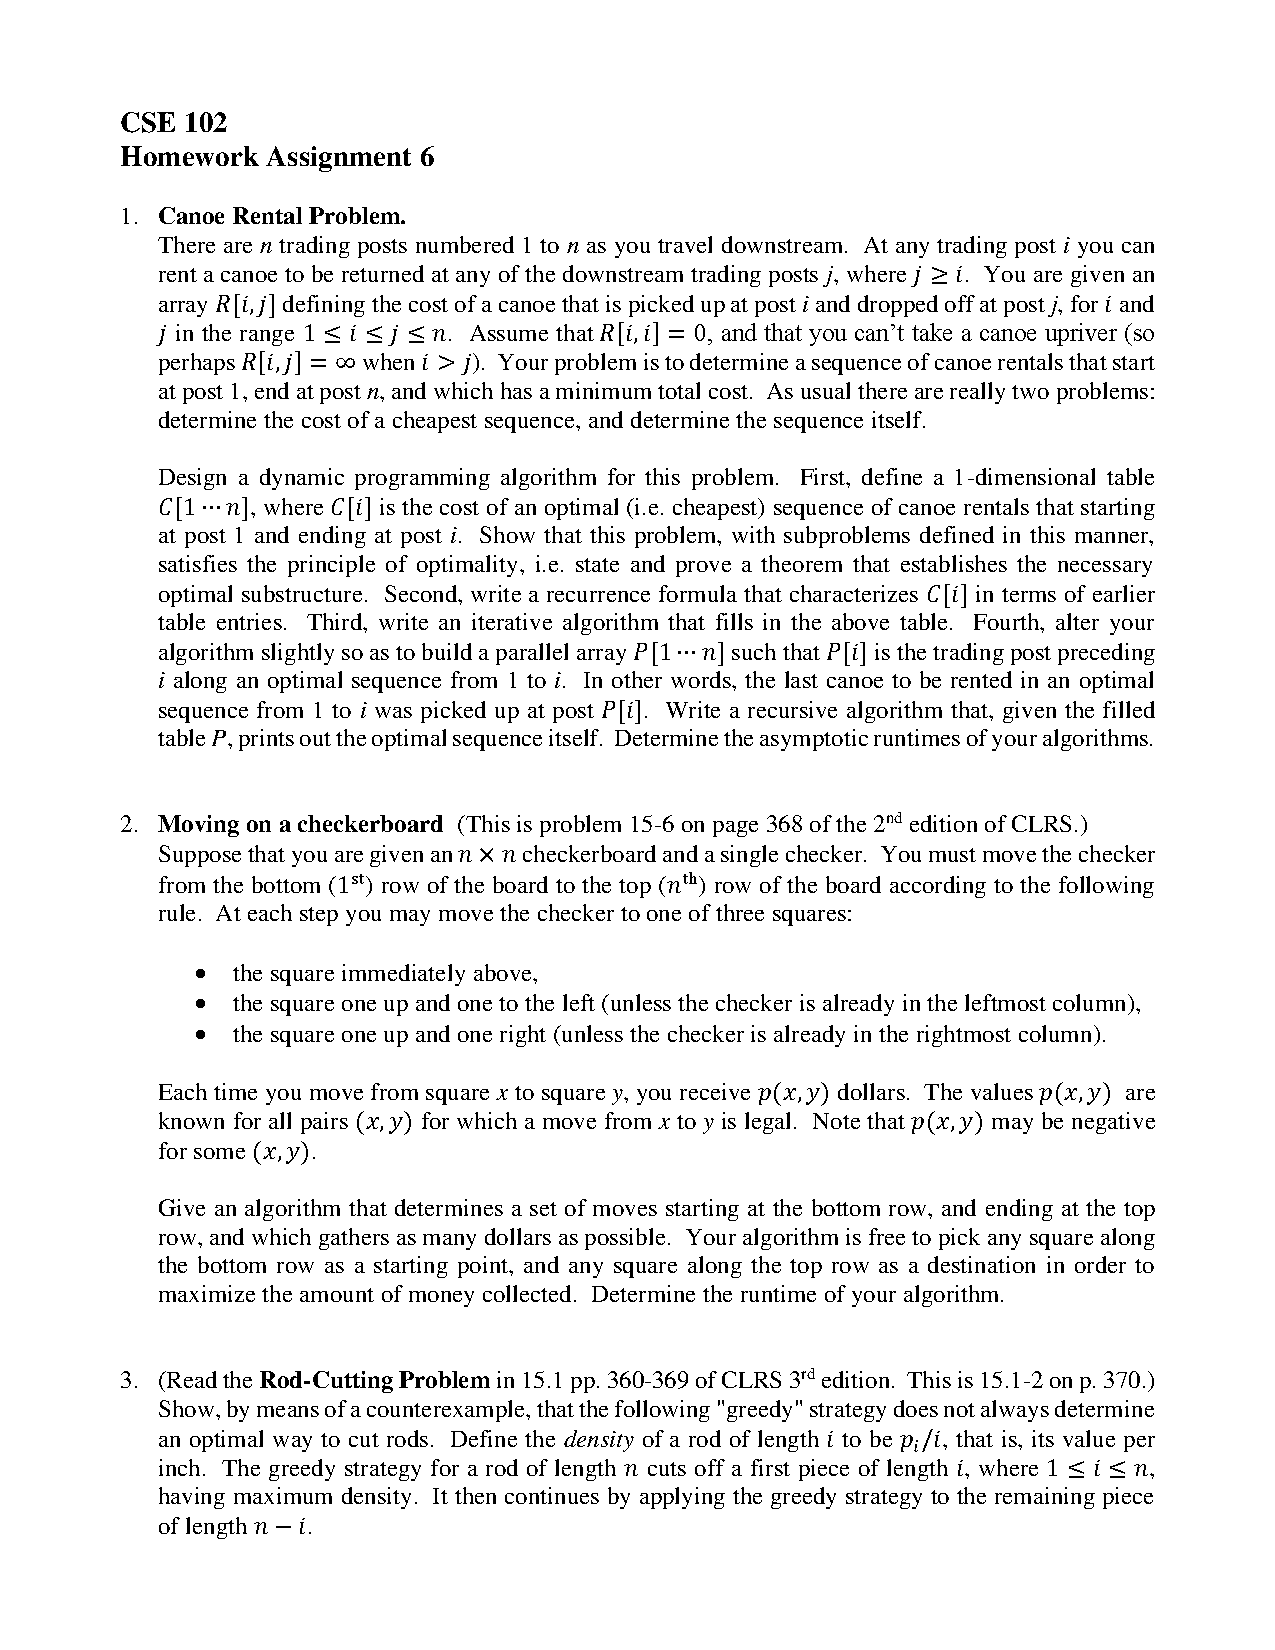
\includepdf[pages=1-1]{homework/hw6.pdf}
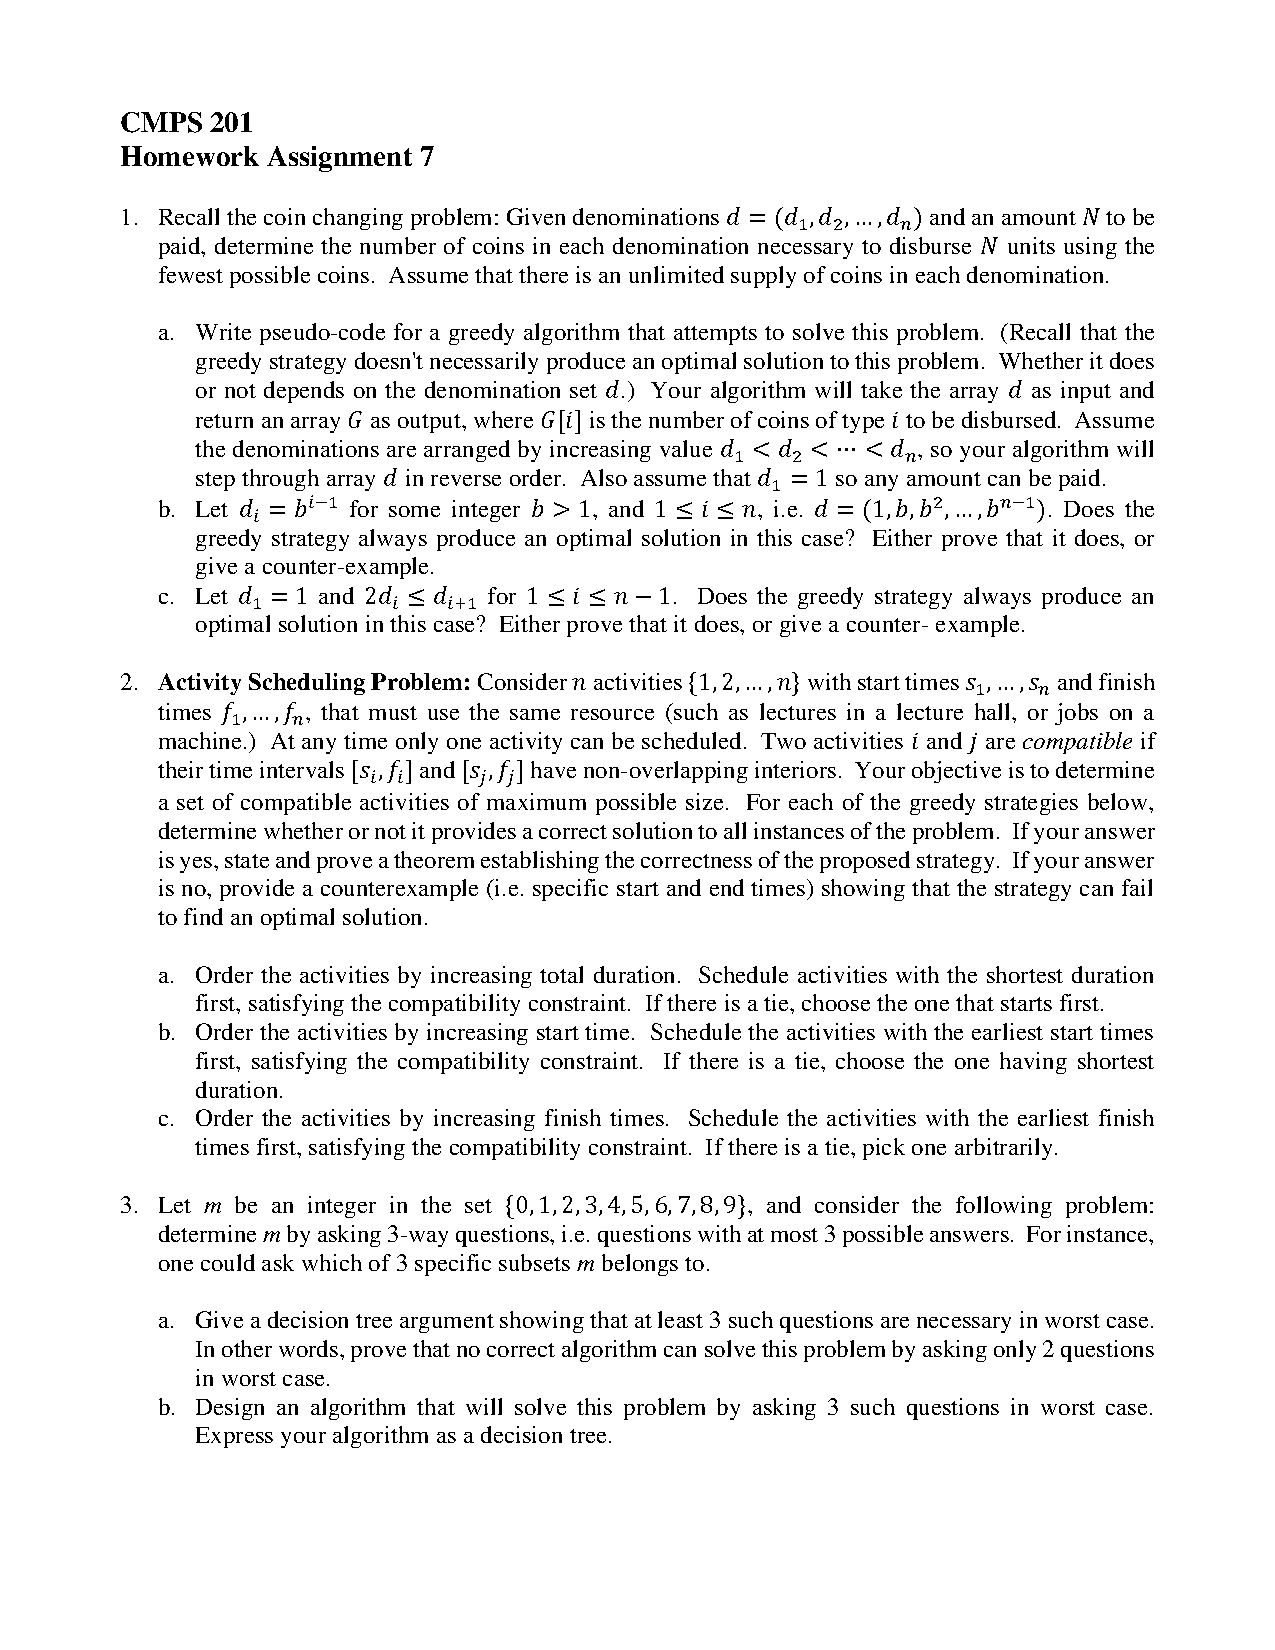
\includepdf[pages=1-2]{homework/hw7.pdf}
\fi
\section{Homework 1 Solutions}

Solutions to Homework assignment 1.

\subsection{Problem 1}

We must prove both $f(n) + g(n) = O(\text{max}(f(n),g(n))$ and $f(n) + g(n) = \Omega(\text{max}(f(n),g(n))$. Assume for this proof $f(n) \ge g(n)$.

$$f(n) + g(n) = O(\text{max}(f(n),g(n))$$
$$= 0 \le f(n) + g(n) \le c_1 \cdot \text{max}(f(n),g(n))$$
$$\text{Let } c_1 = 3 \text{ thus theres is one } n_0, \text{ such that } \forall n \ge n_0 \text{ the inequality above holds.}$$

$$f(n) + g(n) = \Omega(\text{max}(f(n),g(n))$$
$$= 0 \le c_2 \cdot \text{max}(f(n),g(n)) \le f(n) + g(n) $$
$$\text{Let } c_2 = 4 \text{ thus theres is one } n_0, \text{ such that } \forall n \ge n_0 \text{ the inequality above holds.}$$

$$\text{Since } f(n) + g(n) = O(\text{max}(f(n),g(n)) \text{ and } f(n) + g(n) = \Omega(\text{max}(f(n),g(n)) $$
$$f(n) + g(n) = \Theta(\text{max}(f(n),g(n)) \text{ Q.E.D}$$

\subsection{Problem 2}

$$f(n) = \Theta(g(n)) $$
$$\text{For positive constants } c_1 \text{ and } c_2 \text{ and some } n_0, \forall n \ge n_0, \text{ the inequality below is true.}$$
$$= 0 \le c_1 \cdot g(n) \le f(n) \le c_2 \cdot g(n) $$
$$\text{Let us square all sides of the inequality}$$
$$= 0 \le c_1^2 \cdot g(n)^2 \le f(n)^2 \le c_2^2 \cdot g(n)^2 $$
$$\text{Thus for positive constants } c_{1}^2 \text{ and } c_{2}^2 \text{ and some } n_1, \forall n \ge n_1,\text{ the inequality above holds.}$$
$$f(n) = \Theta(g(n) \text{ then } f(n)^2 = \Theta(g(n)^2) \text{ is true. Q.E.D} $$

\subsection{Problem 3}

$$f(n) = \Theta(g(n)) $$
$$\text{For positive constants } c_1 \text{ and } c_2 \text{ and some } n_0, \forall n \ge n_0, \text{ the inequality below is true.}$$
$$= 0 \le c_1 \cdot g(n) \le f(n) \le c_2 \cdot g(n) $$
$$\text{Let us raise all sides of the inequality by base 2}$$
$$= 0 \le 2^{c_1 \cdot g(n)} \le f(n) \le 2^{c_2 \cdot g(n)} $$
$$\text{As seen above } 2^{f(n)} \text{ is still bounded by } 2^{g(n)} \text{ multiplied by two constants.}$$
$$f(n) = \Theta(g(n) \text{ then } 2^{f(n)} = \Theta(2^{g(n)}) \text{ is true. Q.E.D} $$

\subsection{Problem 4}

$$\text{Since } \lim_{n \rightarrow \infty} g(n) = \infty \text{ and } f(n) = \Theta(g(n)) \text{ then } $$
$$\lim_{n \rightarrow \infty} \frac{f(n)}{g(n)} = \frac{\infty}{\infty} = 1$$
$$\text{Then }$$
$$\lim_{n \rightarrow \infty} \frac{\ln(f(n))}{\ln(g(n))} = \frac{\infty}{\infty} = 1$$
$$\ln(f(n)) = \Theta(\ln(g(n)) \text{ Q.E.D}$$

\subsection{Problem 5}

$$\text{Since } \lim_{n \rightarrow \infty} n = \infty \text{ and } f(n) \cdot \ln(f(n)) = \Theta(n) $$
$$\text{Then there are positive constants } c_1 \text{ and } c_2 \text{ and some constant } n_0, \forall n \ge n_0 \text{ that the inequality holds:}$$
$$0 \le c_1 \cdot n \le f(n) \cdot \ln(f(n)) \le c_2 \cdot n$$
$$\text{This shows that } f(n)\cdot\ln(f(n)) \text{ grows at the same rate as n}$$
$$\text{Let us substitute n with } f(n) \text{ this will still hold the inequality}$$
$$0 \le c_1 \cdot f(n) \le f(n) \cdot \ln(f(n)) \le c_2 \cdot f(n)$$
$$\text{Dividing all sides by } f(n) \text{ yields the following inequality:}$$
$$0 \le c_1 \cdot \frac{f(n)}{\ln(f(n))} \le f(n) \le c_2 \cdot \frac{f(n)}{\ln(f(n))}$$
$$\text{Replacing back in n gets us the following inequality:}$$
$$0 \le c_1 \cdot \frac{n}{\ln(n)} \le f(n) \le c_2 \cdot \frac{n}{\ln(n)}$$
$$\text{This shows us that } f(n) \text{ grows at the same rate as } \frac{n}{\ln(n)}$$
$$f(n) = \Theta(\frac{n}{\ln(n)}) \text{ Q.E.D}$$

\subsection{Problem 6a}
Consider $f(c\cdot n) = \Theta(f(n))$ find a function $f(n)$ and constant $c > 0$ such that $f(c \cdot n) \neq \Theta(f(n))$.
$$\text{Let } f(n) = \tan(n) \text{ and } \tan(2n)$$
$$\text{Tangent has periodic behavior along the vertical axis. }$$
$$\text{With 2n, tangent grows faster than n thus not bounded by a constant}$$
$$\tan(2n) \neq \Theta(\tan(n))$$

\subsection{Problem 6b}
Consider $f(c\cdot n) = \Theta(f(n))$ find a function $f(n)$ such that $f(c \cdot n) = \Theta(f(n)), \forall c > 0$.

$$\text{Let } f(n) = n \text{ and } f(c \cdot n) = cn$$
$$\lim_{n \rightarrow \infty} \frac{c \cdot n}{n} = c$$
$$f(c \cdot n) = \Theta(f(n)) \forall c > 0$$

\subsection{Problem 7}

$$\Sigma_{i=1}^{n} a^i = \frac{a(1-a^n)}{1-a}$$
$$\text{If } 0 < a < 1 \text{ then the sum approaches a finite value and thus } \Theta(1)$$
$$\text{If } a = 1 \text{ then the sum is just 1 added n times thus } \Theta(n)$$
$$\text{If } a > 1 \text{ then the sum grows infinity, dominated by } a^n \text{ thus } \Theta(a^n)$$

\subsection{Problem 8}

$$\text{Prove by induction: } \Sigma_{k=1}^{n} k^4 = \frac{n(n+1)(6n^3 + 9n^2 + n - 1)}{30} \text{ for all } n \ge 1$$
$$\text{Base case: } n = 1 $$
$$\Sigma_{k=1}^{1} k^4 = \frac{1(1+1)(6+9+1-1)}{30}$$
$$= \frac{2\cdot15}{30}$$
$$= 1 $$
$$\text{Inductive Hypothesis: } n = n$$
$$\Sigma_{k=1}^{n} k^4 = \frac{n(n+1)(6n^3 + 9n^2 + n - 1)}{30}$$
$$\text{Inductive Step: } n = n+1$$
$$\Sigma_{k=1}^{n+1} k^4 = 1 + 16 + 81 + \dots + n^4 + (n+1)^4$$
$$= \frac{n(n+1)(6n^3 + 9n^2 + n - 1)}{30} + (n+1)^4$$
$$= \frac{n(n+1)(6n^3 + 9n^2 + n - 1) + 30(n+1)^4}{30} $$
$$= \frac{n(n+1)(6n^3 + 9n^2 + n - 1) + 30(n+1)(n+1)^3}{30} $$
$$= \frac{n(n+1)(6n^3 + 9n^2 + n - 1) + (n+1)(30n^3 + 90n^2 + 90n +30)}{30} $$
$$= \frac{n(n+1)(6n^3 + 9n^2 + n - 1) + n(n+1)(30n^2 + 90n^1 + 90 + \frac{30}{n})}{30} $$
$$= \frac{n(n+1)(6n^3 + 9n^2 + n - 1 + 30n^2 + 90n + 90 + \frac{30}{n})}{30} $$
$$= \frac{n(n+1)(6n^3 + 39n^2 + 91n + 89 + \frac{30}{n})}{30} $$
$$= \frac{(n+1)(6n^4 + 39n^3 + 91n^2 + 89n + 30)}{30} $$
$$\text{Factor out } n + 2 \text{ by long polynomial division from } 6n^4 + 39n^3 + 91n^2 + 89n + 30 \text{.}$$
$$= \frac{(n+1)(n+2)(6n^3 + 27n^2 + 37n + 15)}{30} $$
$$\text{Rearrange some terms.}$$
$$= \frac{(n+1)(n+2)(6n^3 + 18n^2 + 18n + 6 + 9n^2 + 18n + 9 + n)}{30} $$
$$= \frac{(n+1)(n+2)(6(n+1)^3 + 9(n+1)^2 + n)}{30} $$
$$= \frac{(n+1)((n + 1) + 1)(6(n+1)^3 + 9(n+1)^2 + (n + 1) - 1)}{30} $$
$$\text{Q.E.D}$$



\end{document}